\chapter{All-sky Analysis}
  \label{ch:allsky}
    What we present here is a test of the generalizability of results from Ch.\ref{ch:lori}, which focused on a particular structure on the sky, $\lambda$~Orionis.
    We first would like to note that ``all-sky analysis'' can be a bit misleading. The term tends to lead readers to the idea of a definitive study, answering a particular question for any given position on the sky.  While a truly all-sky analysis would be ideal, signal-to-noise constraints (mainly at high galactic latitudes), as well as confusion along the line of sight (mainly in the galactic plane), make a uniformly powerful study of the whole sky very challenging. Here we will indeed show results for the entire sky as a benchmark analysis, but for the core analysis we must mask certain regions dominated by systematic effects in order to minimize biases for particular wavelenghts.

\section{Resolution matching}
    \subsubsection{Smoothing}
        As in Ch.~\ref{ch:lori}, this approach applies to a spatial resolution of approximately \textasciitilde{}$1^{\circ}$. The resolution limimtation is imposed by the \gls{pc} microwave component maps, which list an effective resolution of 60$'$ \citep{planck15X}. Thus we must apply a smoothing to most of our input datasets, which have native resolutions of a much finer scale (see Tab.~\ref{tab:data} and Fig.~\ref{fig:AME_contours}). The data also come in a wide range of beam shapes with their own degrees of uncertainty, thus we conservatively smooth all of the data in the same way, using a circular Gaussian beam, to have \textasciitilde{}$1^{\circ}$ FWHM resolution. We start with an all-sky \gls{ame} to IR comparison, looking for global patterns among all pixels.

    \subsubsection{Offset correction}
    In Ch.~\ref{ch:lori}, we utilized the latest available version of the AKARI/\gls{irc} data. However, the latest version is still undergoing final processing for some parts of the sky, at the time of this analysis. Thus we must use a previous version for this all-sky analysis. The major difference between the previous version, and that used in Ch.~\ref{ch:lori}, is an apparent all-sky positive offset of \textasciitilde{}2~MJy/sr for A9 and \textasciitilde{}5~MJy/sr for A18. We assess this offset first by finding the mode of each of the 4,737 $3^{\circ}\times3^{\circ}$ tiles of the IRC survey, for each band, and then taking the mode of that distribution. This distribution of tile modes is shown in Fig.~\ref{fig:allsky_2016_tilemodes}.
        \begin{figure}
          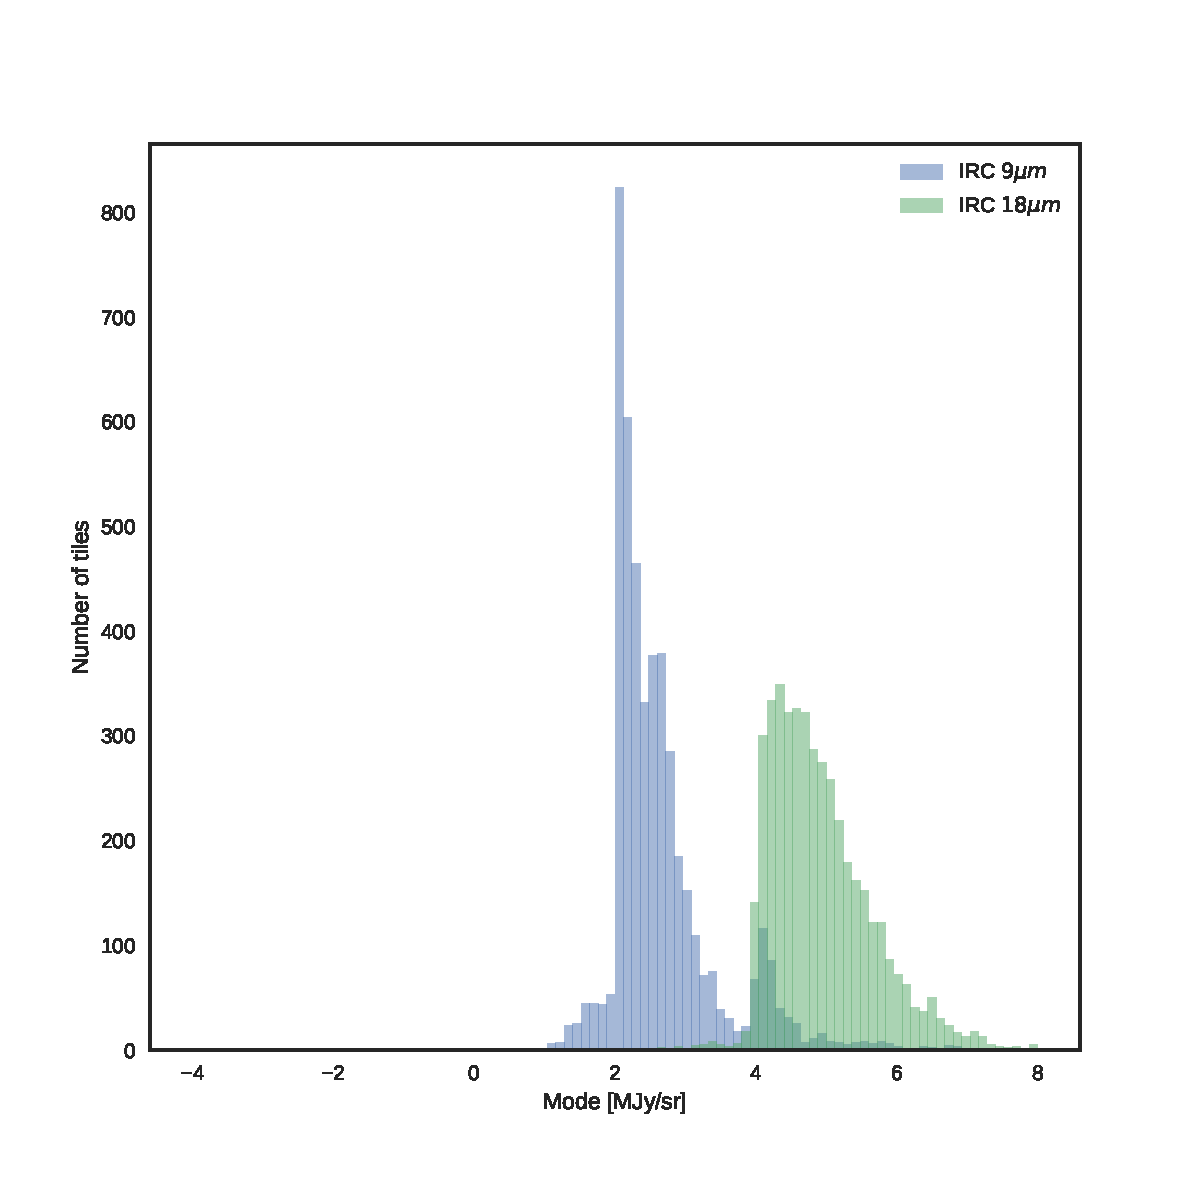
\includegraphics[width=\textwidth]{../Plots/ch_allsky/IRC_offset_correction.pdf}
          \centering
          \caption{Distributions of the modal values for each of the 4,737 survey tiles for the A9 band, and for the A18 band.}
          \label{fig:allsky_2016_tilemodes}
        \end{figure}
      We then compare this result with a monopole offset fit to the all-sky HEALPix map of the IRC surveys, built from these tiles. Monopole fitting is handled by the {\tt healpy.fit\_monopole} function.
      The monopole values subtracted from each map shown in Tab.~\ref{tab:allsky_monopoles}.
         \begin{table}
           \caption{Monopole values subtracted from all-sky HEALPix maps}
           \centering
             \begin{tabular}{lr}
               \hline\hline
               Map & Monopole \\
                  &  [MJy/sr] \\
               \hline
               \centering
               A9  & 2.27 \\
               A18 & 5.10 \\
               A65 & 1.96 \\
               A90 & 3.13 \\
               A140 & 4.64 \\
               A160 & 4.65 \\
               I12 & 1.00 \\
               I25 & 1.79 \\
               I60 & 0.77 \\
               I100 & 3.04 \\
               P857 & 1.92 \\
               P545 & 0.68 \\
               \hline
               \label{tab:allsky_monopoles}
            \end{tabular}
         \end{table}

      We find the values produced by these two methods to be consistent. We found offsets also in the \gls{iras}, \gls{fis}, and \gls{hfi} bands, thus we apply the same monopole fitting and subtraction to all of the all-sky maps. We do not find the correlation analysis presented in later sections to be sensitive to this offset correction.

  \section{All-sky cross correlations}
        In order to look more closely at how the \gls{ame} to \gls{ir} relationship varies with wavelength, we first do a comparison without applying any pixel mask, as a benchmark. Fig.~\ref{fig:AMEvsDust_allsky_allbands_mpsub_kde_unmasked} shows the pixel-density plots of \gls{ame} vs. the IR bands' intensities. Darker regions show higher pixel densities, unshaded or more lightly shaded regions show low or zero pixel densities. An intial analysis, considering only the interreations of the \gls{pc} parameter maps, was presented in Sec.~\ref{sec:PCmaps}, wherein correlations between the major microwave component maps (synchrotron, free-free, \gls{ame}, and dust emisison) are demonstrated (Fig.~\ref{fig:PCCS_corrmatrix}). This section extends that analysis, considering the full range of IR maps described in Tab.~\ref{tab:data}.

        We see immediately that each band shows evidence of a positive trend with \gls{ame} intensity. For the \gls{mir} bands, at lower IR intensities we see the effects of detector noise become dominant, turning into a more defined positive trend with increasing IR intensity. This effect is less pronounced in the FIR. The trend is similar to that found in Ch.~\ref{ch:lori}, and Fig.~\ref{fig:orionis-corr-matrix}.
          \begin{figure}
            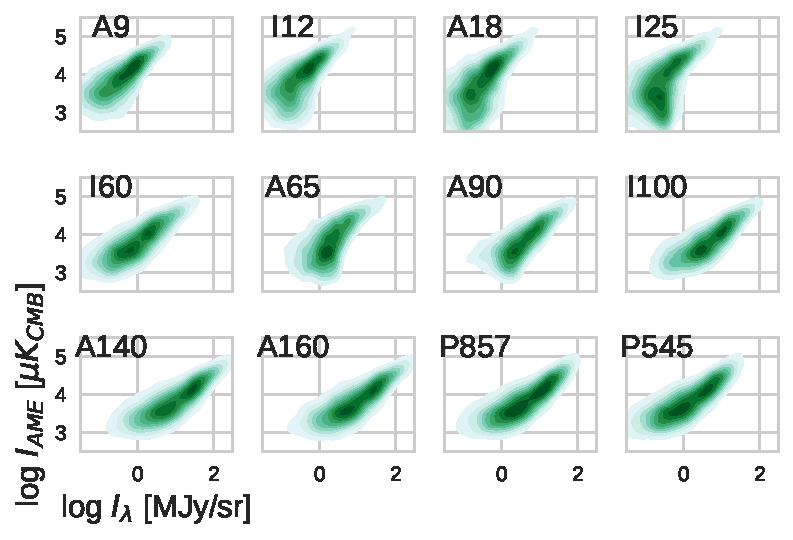
\includegraphics[width=\textwidth]{../Plots/ch_allsky/AMEvsDust_allsky_allbands_mpsub_kde_unmasked.pdf}
            \centering
            \caption{Point-density distributions of the log $AME_{var}$ intensity (Y-axis) vs. log IR bands' intensities. In this case no pixel mask is applied, in order to show overall trend of the full data-set. However a random sampling is used due to computational contraints. The plots show a random set of 20\% of the full-sky data. Darker shaded regions indicate a higher density of pixels.}
            \label{fig:AMEvsDust_allsky_allbands_mpsub_kde_unmasked}
          \end{figure}
        We consider that the IR maps used must not only be compared to the \gls{ame}, but to each other, to assess multi-wavelength patterns. We also compare the \gls{ame} and IR maps to ancilliary maps, as described in Ch.~\ref{ch:datasources} and Tab.~\ref{tab:ancilliarydata}. Fig.~\ref{fig:all_bands_corr_matrix_wAME_spearman} confirms the weaker trend in the \gls{mir} vs. \gls{ame}, via a cross-correlation matrix, similar to that used in Ch.~\ref{ch:lori} and Fig.~\ref{fig:orionis-corr-matrix}.
          \begin{figure}
            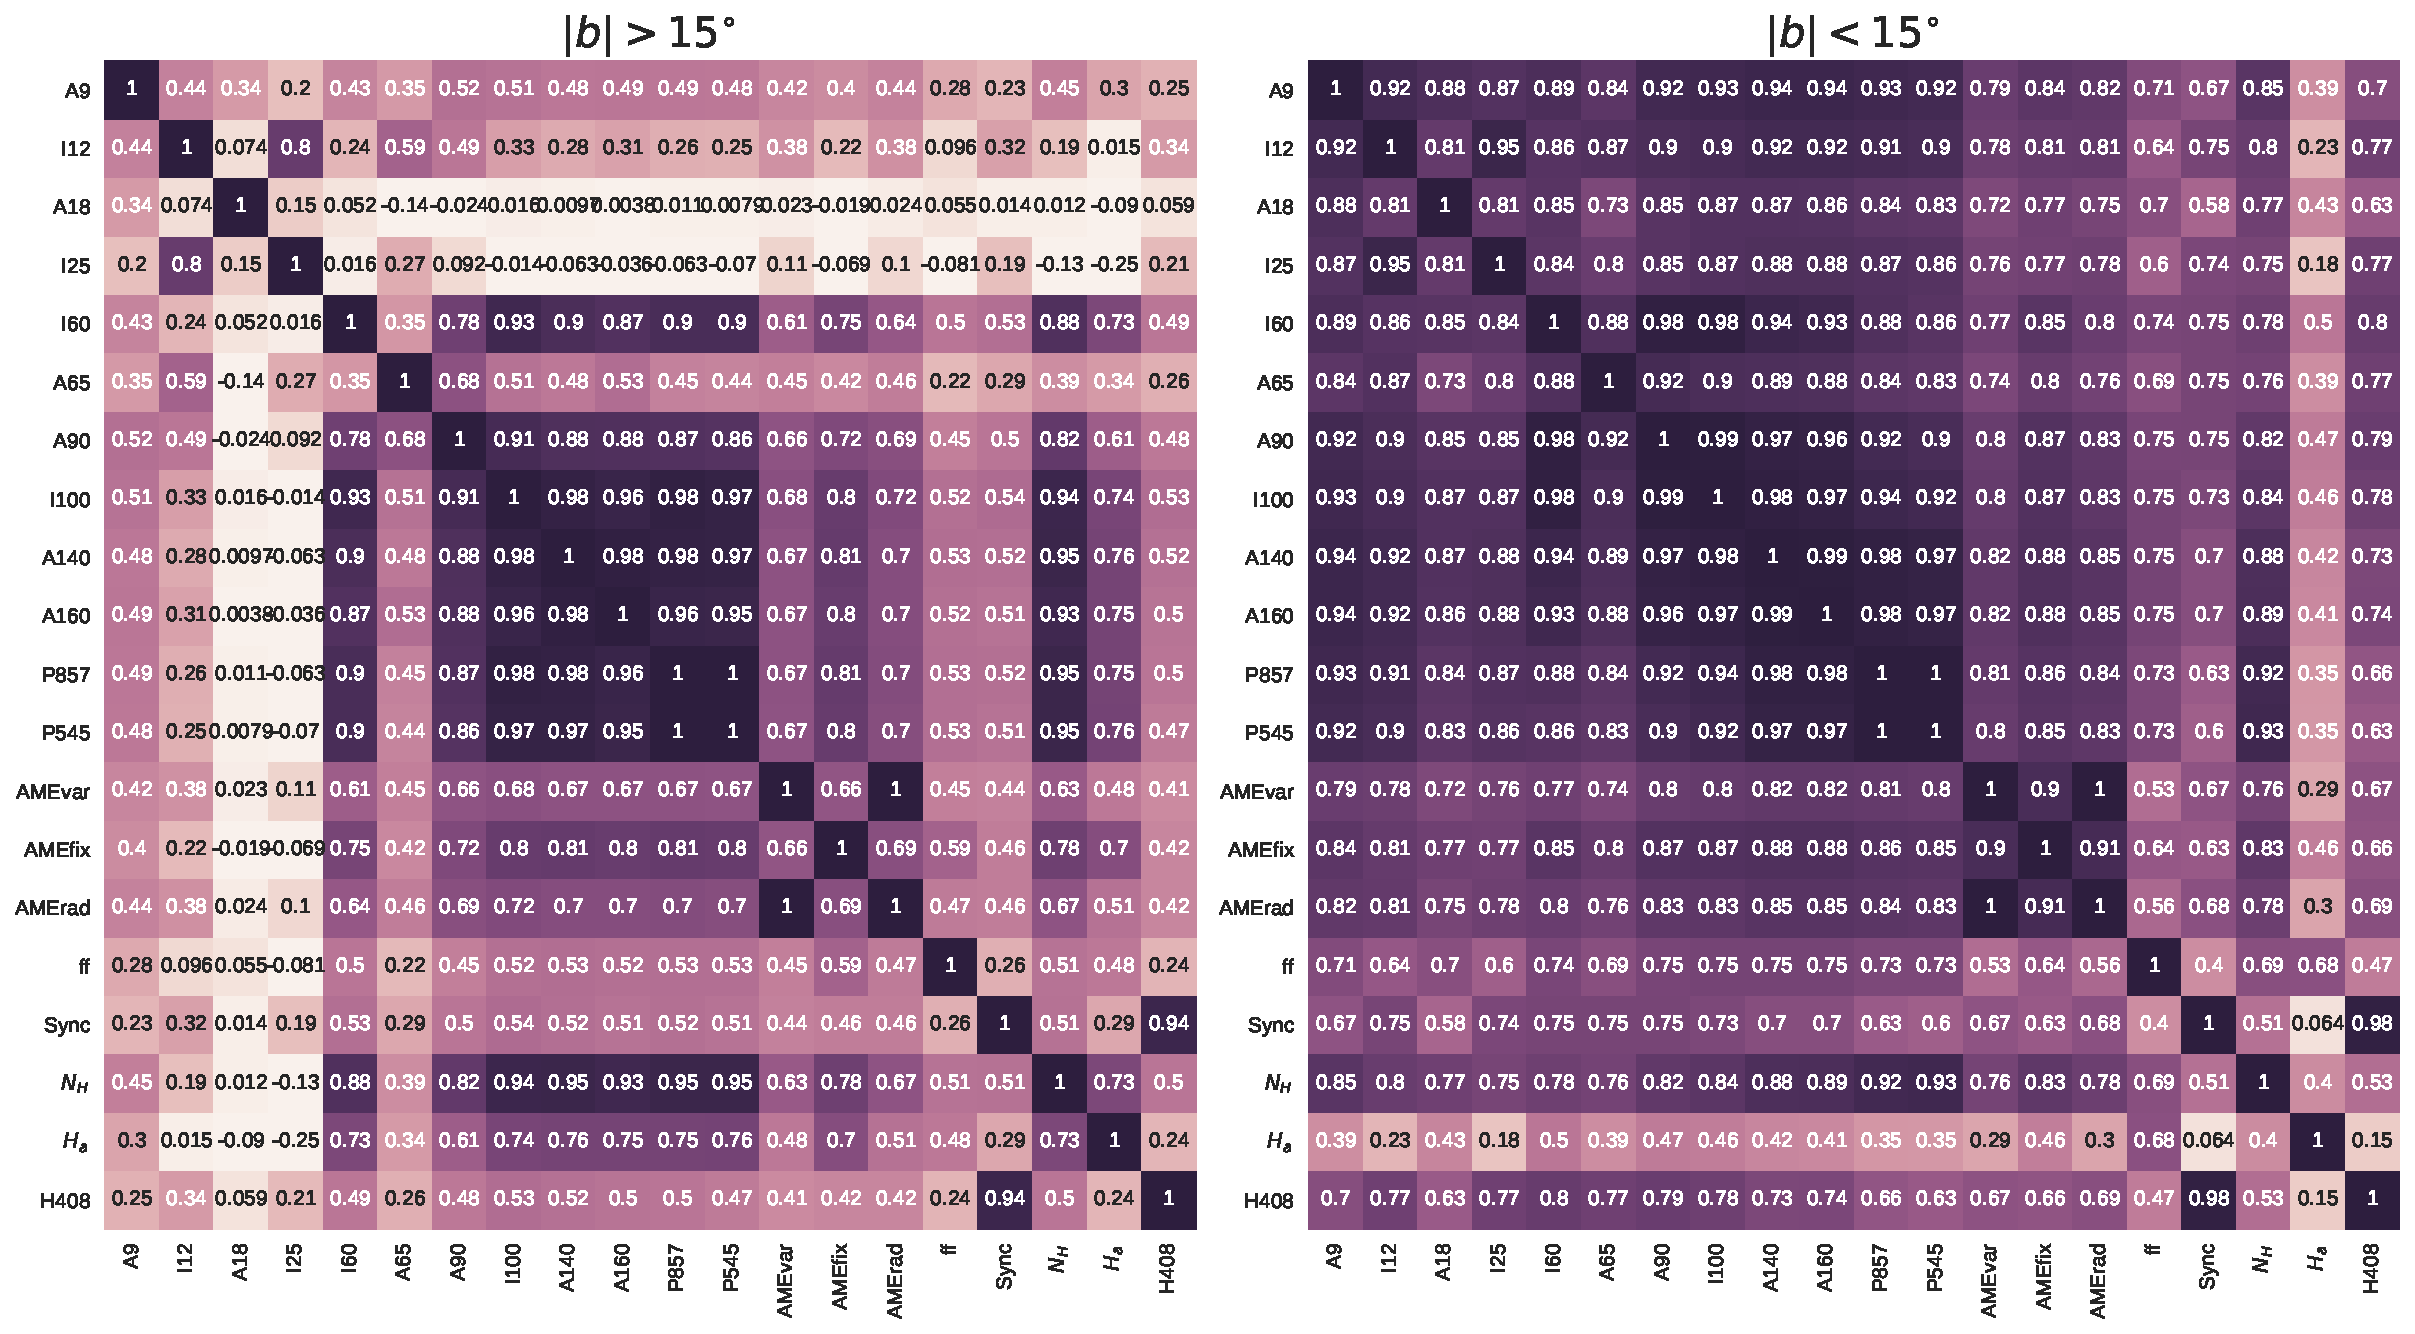
\includegraphics[width=\textwidth]{../Plots/ch_allsky/all_bands_corr_matrix_wAME_spearmanintensity_unmasked.pdf}
            \centering
            \caption{ALL-SKY cross-correlation matrix for the 12 infrared bands sampled, as well as the PC component maps described in Ch.~\ref{ch:datasources}: the two \gls{ame} components evaluated at their peak frequencies $AME_{var}$, $AME_{fix}$; Syncrotron, and free-free), and ancilliary maps of $N_{H}$, $H{\alpha}$ emission, and 408~MHz emission \cite{haslam82}. The color-scale indicates ($r_{S}$). Results are based on the unmasked sky, but are split by Galactic latitude: pixels with $|\beta{}| > 15^{\circ}$ (left) and $|\beta{}| < 15^{\circ}$ (right). The color and annotations indicate $r_{s}$ as in Fig.~\ref{fig:orionis-corr-matrix}. }
            \label{fig:all_bands_corr_matrix_wAME_spearman}
          \end{figure}
       This is reflected in the comparison between high and low latitude plots: for pixels $|\beta| > 15 ^{\circ}$, we see a dramatic effect. In the most extreme case $r_{s}$ of A18 to $AME_{var}$ drops from 0.72 at lower latitudes, to 0.02 at higher latitudes. $r_{s}(A9:AME_{var})$ drops from 0.79 to 0.42. Correlations between the \gls{mir} bands and FIR bands also weaken. Only the the interrelations between the FIR bands from I60 to P545 remain essentially latitude independent (with the exception of A65, which has an especially high noise level.)

        In the lower latitudes, with $|\beta| < 15^{\circ}$, bright emission in and around the galactic plane seems to homogenize the bands. We see little change from band to band both in terms of the relationship with \gls{ame} or with other IR bands. Thus the increase of \gls{sn} with decreasing brightness at higher latitudes has a strong effect on such intensity correlation tests. Bands tracing bright thermal dust emission at higher latitudes are more robust against this effect. The only case where the trend is reversed, is with the maps of $N(H)$ and $H{\alpha}$. Both of these maps show higher $r_{s}$ when compared to high latitude FIR emission, possibly due to optical effects. The next section descibes a pixel-masking strategy designed to mitigate both $r_{s}$ suppressing effects from band-to-band \gls{sn} variations, and $r_{s}$ enhancing effects from confusion near the galactic plane.

      \section{Masked Comparison}
        For the reasons described in the previous section, we consider that an exhaustive comparsion of the \gls{ame} with IR requires the use of a pixel mask. In this section we describe the various masks applied to the full dataset. We then repeat both the comparisons above (as in  Figs.~\ref{fig:AMEvsDust_allsky_allbands_mpsub_kde_unmasked} and~\ref{fig:all_bands_corr_matrix_wAME_spearman}) for the masked dataset, and present additional analyses. The full mask, superimposed on A9 map, is shown in Fig.~\ref{fig:A9_masked_map}, with the details of the mask layers desribed in the next subsection. The mask most heavily affects high galactic latitudes, and the galactic plane. The same mask is applied to all of the maps.
          \begin{figure}
            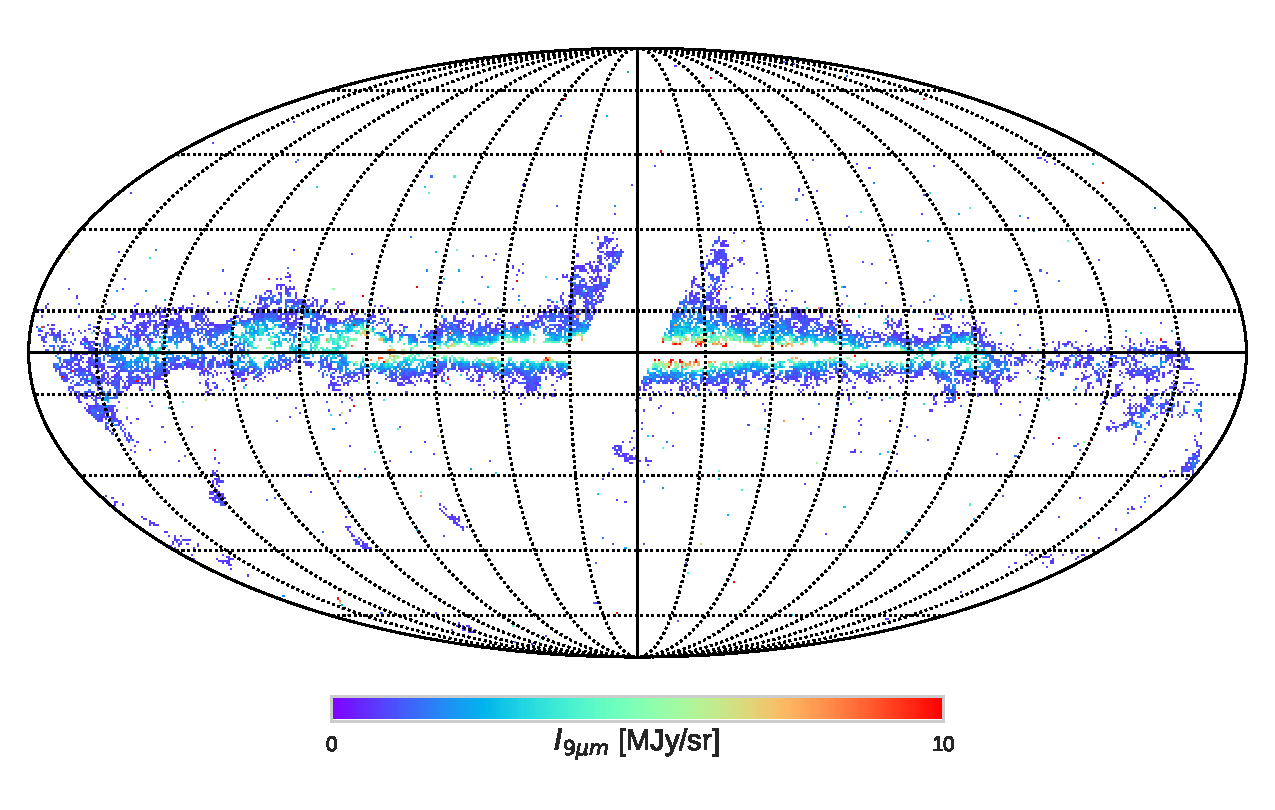
\includegraphics[width=\textwidth]{../Plots/ch_allsky/masked_map_A9.pdf}
            \centering
            \caption{All-sky map in A9 emission after applying the combined masks: ecliptic plane, galactic plane, point sources, and pixels with \gls{sn} $<3$. This mask essentially outlines the galaxy, except for the most confused regions. Diffuse galactic emission is essentially removed by the mask due to low \gls{sn} in the \gls{mir} bands. In the full sky map of \textasciitilde{}700,000 pixels, there are \textasciitilde{}50,000 unmasked pixels remaining.}
            \label{fig:A9_masked_map}
          \end{figure}

      \subsection{Pixel mask}
      \label{sec:pixmask}
        \paragraph{Galactic plane}
          The galactic plane tends to be a challenge in any comparison, but especially with low resolutions studies such as the present work. Complicated structures along the line of sight, smoothed to $1^{\circ}$ resolution, means that emisison within any given pixel is an average of many different environments (evidenced by the homogenizing of the correlations between bands at low latitudes in Fig.~\ref{fig:all_bands_corr_matrix_wAME_spearman}.) Thus we exclude the brightest emission of the galactic plane, according to the mask prepared by the Planck Collaboration.

        \paragraph{Zodiacal light}
          To minimize the effects of residual zodiacal light, we exclude pixels within $10^{\circ}$ of the ecliptic plane.  Even though we use the Zodi-subtracted maps \citep{kelsall98, kondo16, ootsubo16}, the Zodi residuals are still problematic (especially in the MIR.) This corresponds to regions with the heaviest contamination from Zodiacal light, where Zodi residuals are apparent even with visual inspection for all of the \gls{mir} bands used in this study. In Ch.~\ref{ch:datasources}, Figs. \ref{fig:ratioMap_A9I12}, and \ref{fig:ratioMap_A9I12} clearly display these residual patterns.

        \paragraph{Signal to noise}
          Some of the bands used lack sufficient sensitivity to trace fainter emisison, especially at higher galactic latitudes. This is mainly an issue for the mid-infrared bands. As such, we enforce a 3$\sigma$ threshold for all of the maps--- adding to the mask any pixel that has lower than 3$\sigma$ detection in any of the maps. This removes nearly all pixels beyond approximately $15^{\circ}$ from the galactic plane, with the pronounced exception of regions affected by stray moonlight. The extent of this particular mask is primarily defined by the IRC A9 and A18 maps, which have the highest noise levels.

       \paragraph{Point Sources}
         The Planck Collaboration provides masks of the pixels they find to include point sources. We mask pixels which are flagged as being point-source contaminated, in the most heavily affected maps: Planck/HFI~857 GHz and Planck/LFI~30 GHz.

      \paragraph{PC Component Separation Errors}
        As noted in \cite{planck15X, hensley16}, there are fluctuations in the PC maps wherein \gls{ame} emission appears to correspond to fluctuations in the synchrotron map. While a mask of all but the most reliably component separated pixels would be ideal, the construction of such a mask with the current data would require us to use a rather artificial threshold. While PC does provide error maps for each of the components, these are not necessarily an indication of how confident the component separation process itself is at a given pixel. We prefer not to apply any additional masks tailored to the PC maps, and instead present and discuss the results with the possibility of component separation artifacts in mind. However we do note that applying the LFI point source mask and galactic plane masks serves also to mask most pixels with \gls{ame} peak frequency outliers.

        \subsection{Effect of mask application}
            Fig.~\ref{fig:AMEvsDust_allsky_allbands_mpsub_kde_masked} shows point-density plots for $AME_{var}$ vs. each of the IR bands, after applying the mask described above.
               \begin{figure}
                 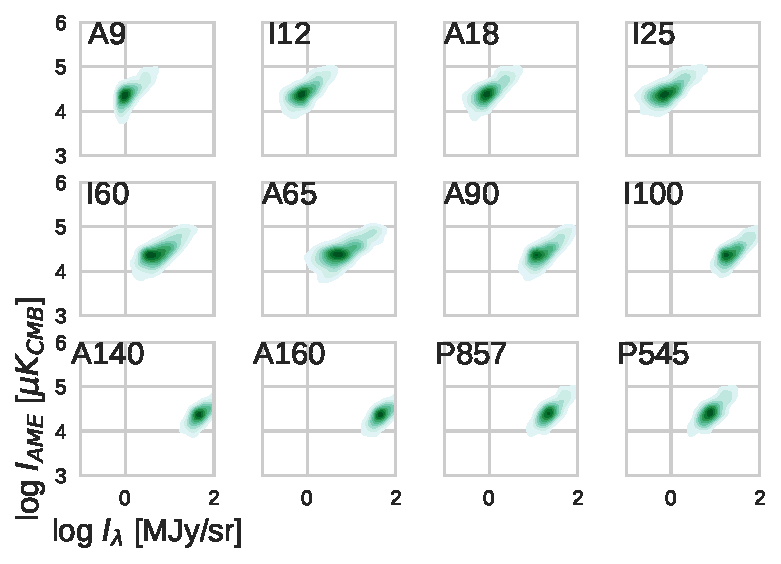
\includegraphics[width=\textwidth]{../Plots/ch_allsky/AMEvsDust_allsky_allbands_mpsub_kde_masked.pdf}
                 \centering
                 \caption{The same comparison as shown for Fig.~\ref{fig:AMEvsDust_allsky_allbands_mpsub_kde_unmasked}, but with the mask applied as in Fig.~\ref{fig:A9_masked_map}.}
                 \label{fig:AMEvsDust_allsky_allbands_mpsub_kde_masked}
               \end{figure}
            This reduces the number of pixels from \textasciitilde{}780,000 to \textasciitilde{}50,000, with about 7\% of the sky remaining. As expected with such a drastic reduction of the number of noise-dominated points, the scatter, especially for the \gls{mir} bands, is reduced. This can be seen by comparing Fig.~\ref{fig:AMEvsDust_allsky_allbands_mpsub_kde_masked} to the unmasked distributions vs. \gls{ame} in Fig.~\ref{fig:AMEvsDust_allsky_allbands_mpsub_kde_unmasked}. Otherwise the applicaiton of the mask does not bring about any special distinction among the bands when compared to the \gls{ame}. What is notable however is that the persistent weakening of trend of I25 vs. \gls{ame}, relative to A9 and the FIR bands. This is seen also when looking at the full set of interrelations via the cross-correlation matrix in Fig.~\ref{fig:all_bands_corr_matrix_wAME_spearmanintensity_maskall}.
              \begin{figure}
                 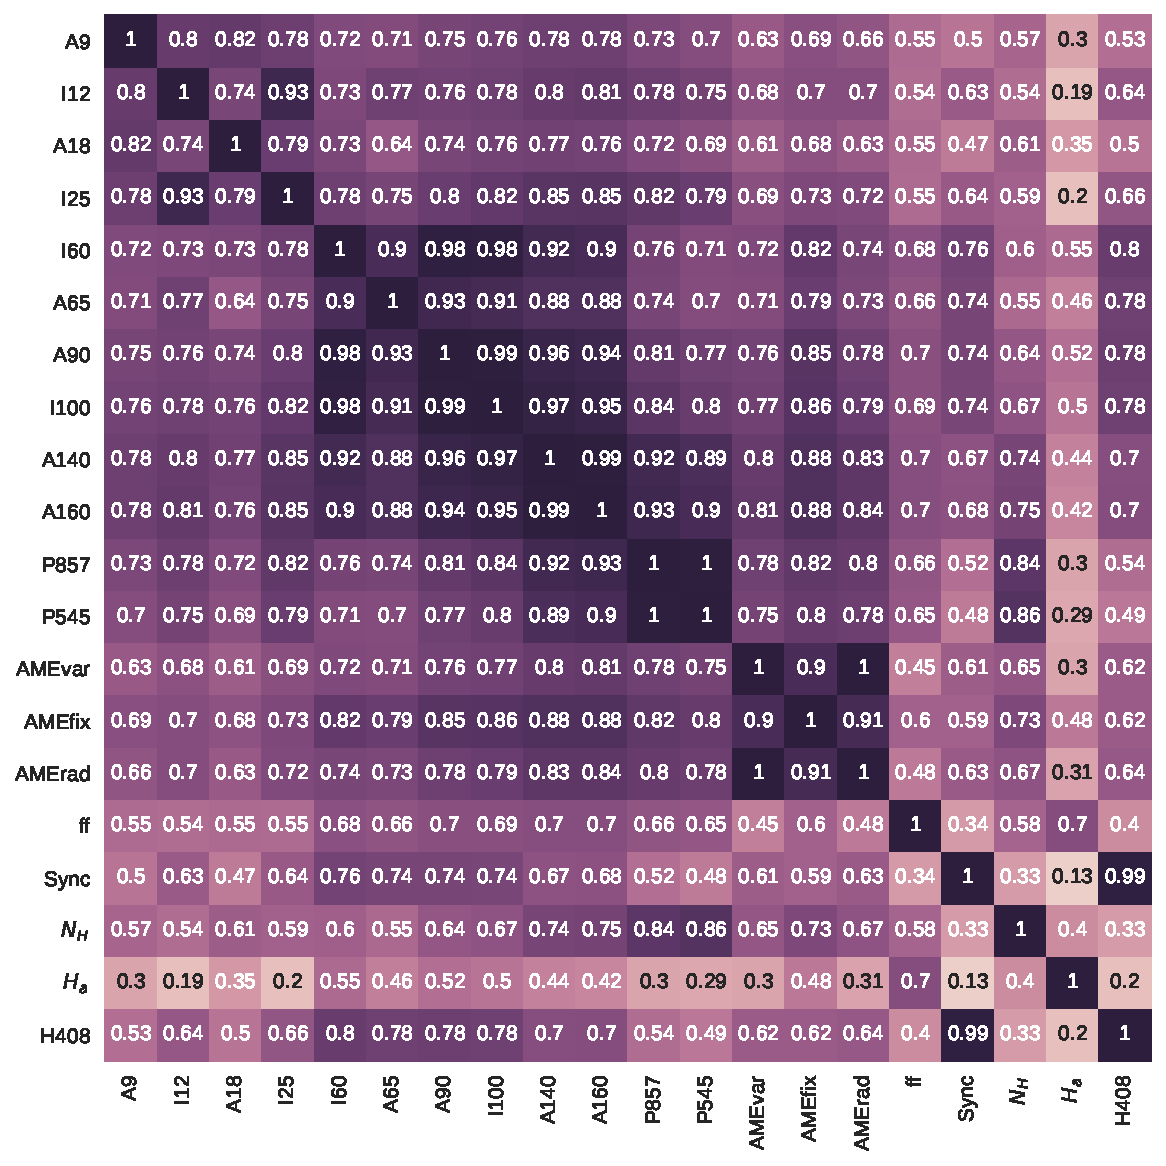
\includegraphics[width=\textwidth]{../Plots/ch_allsky/all_bands_corr_matrix_wAME_spearmanintensity_maskall.pdf}
                 \centering
                 \caption{Cross-correlation ($r_{s}$ matrix for the IR intensities (unscaled) vs. each other, esssentially the same comparison as in Fig.~\ref{fig:all_bands_corr_matrix_wAME_spearman}, except that the pixel mask is applied, and we do not perform a split by Galactic latitude--- after the mask is applied, over 90\% of pixels are within $10^{\circ}$ of the galactic plane.}
                 \label{fig:all_bands_corr_matrix_wAME_spearmanintensity_maskall}
              \end{figure}

        \paragraph{Normalizing by radiation field $U$}
          Following the logic that the \gls{pah}-tracing bands intensity is essentially a product $U$ and the column density of \gls{pah}s $\sigma_{PAH}$ (as explained in Ch.~\ref{ch:datasources}), we redraw the comparison after scaling the \gls{mir} bands by $U$. We determine $U$ by taking the $1^{\circ}$-smoothed, degraded PR1 dust radiance map (also used in \citep{hensley16}), and its corresponding $\tau_{353}$ map. We approximate $U \propto R/\tau_{353}$. In the case of $U$-normalized intensities correlation plots, we only include the \gls{mir} bands. While $I_{MIR}/U$ is thought to trace column density of the band carriers (PAHs, or VSGs), there is a less definite interpretation of $I_{FIR}/U$ (since the profile of FIR dust emission depends on the dust temperature.) Thus for this particular comparison, we represent the FIR with $\tau_{353}$. The $U$-normalized correlation matrix is given by Fig~\ref{fig:all_bands_corr_matrix_wAME_spearmanU_norm_masked}.
                \begin{figure}
                    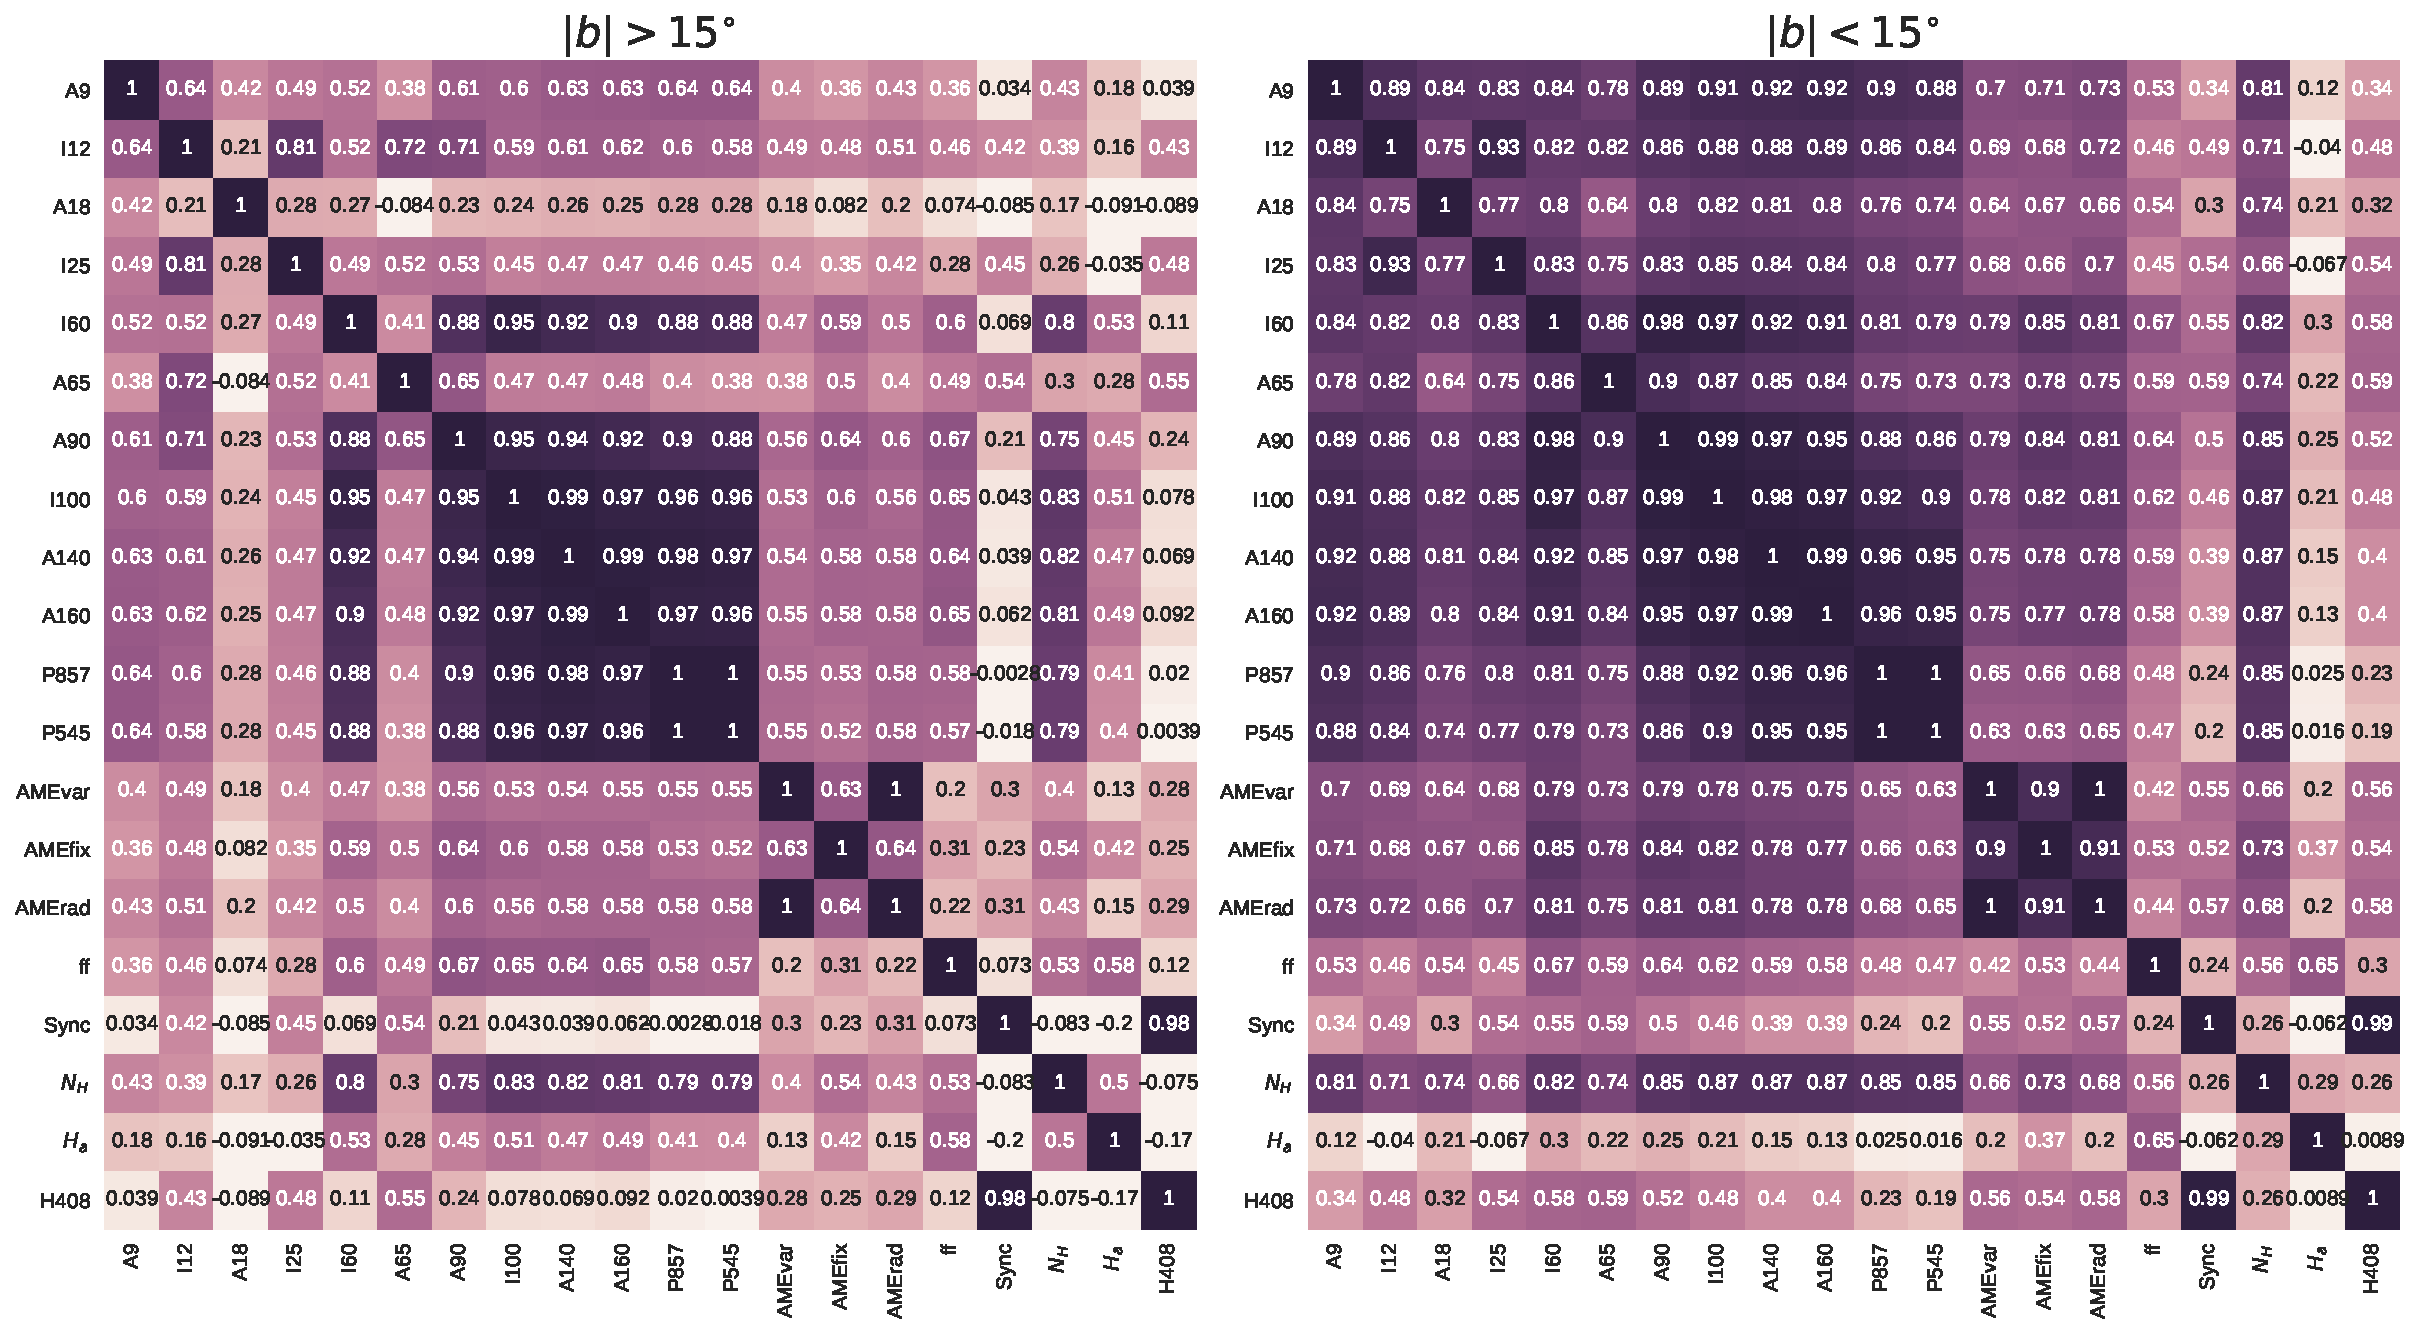
\includegraphics[width=0.49\textwidth,trim={0.2cm 0 0.25cm 0 },clip]{../Plots/ch_allsky/all_bands_corr_matrix_wAME_spearmanU_norm_masked.pdf}
                    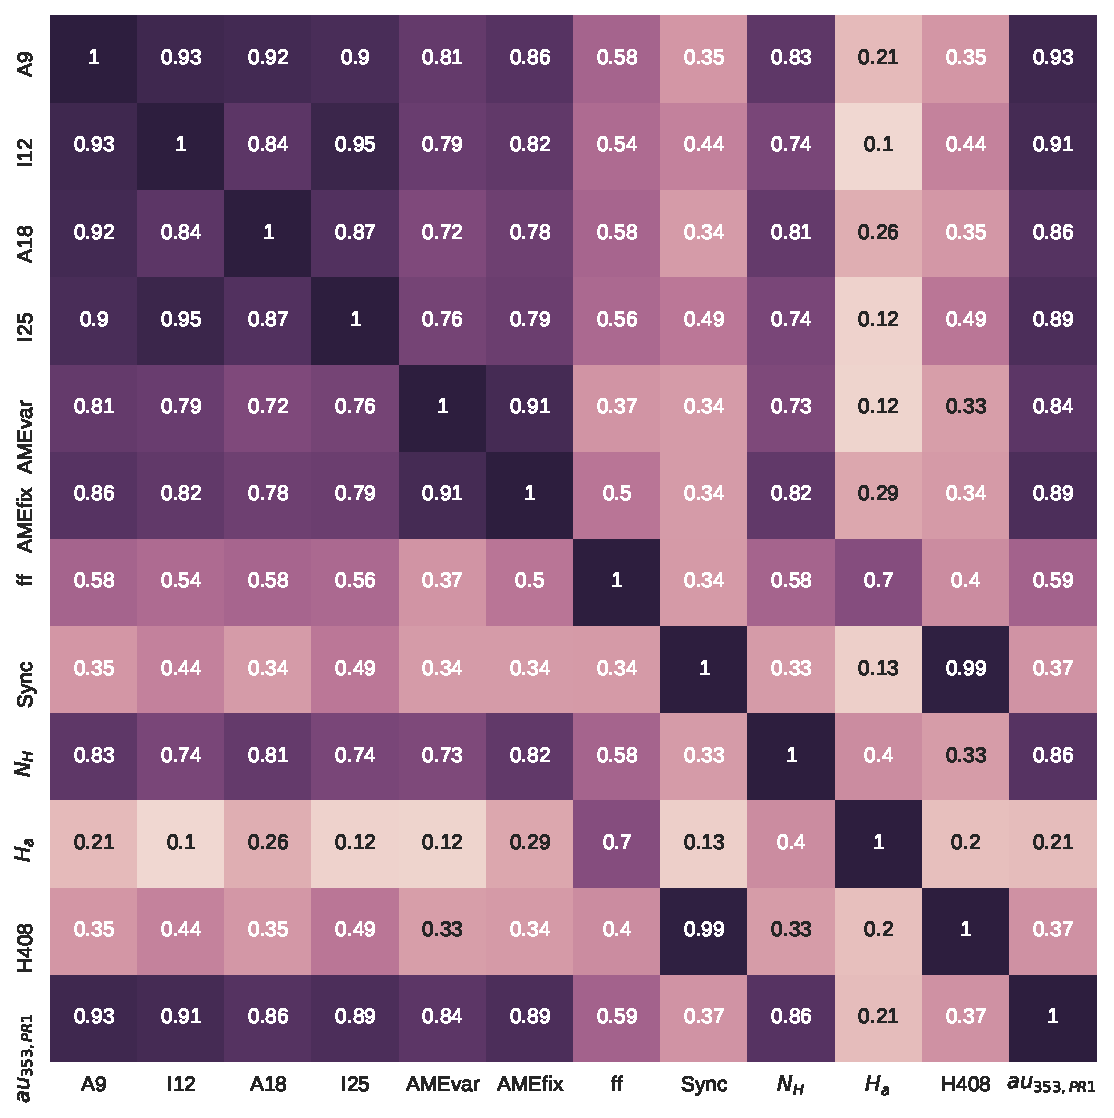
\includegraphics[width=0.49\textwidth,trim={0.2cm 0 0.25cm 0 },clip]{../Plots/ch_allsky/all_bands_corr_matrix_wAME_spearmanU_norm_AMEnorm_masked.pdf}
                    \centering
                    \caption{Cross-correlation ($r_{s}$ matrix for the $U$-normalized IR intensities vs. each other, and also against the \gls{ame} components, other PC products, and ancilliary data. In the left panel, only the IR maps are divided by $U$- other data is unchanged from. In the panel at right, both the the \gls{ame} and IR intensities are divided by $U$. Fig.~\ref{fig:all_bands_corr_matrix_wAME_spearmanintensity_maskall})}
                    \label{fig:all_bands_corr_matrix_wAME_spearmanU_norm_masked}
                \end{figure}
            In this comparison, we see that all of the correlations of the \gls{mir} bands vs. \gls{ame} weaken slightly when we scale the \gls{mir} bands by $U$. However if we consider that $U$ may also affect the \gls{ame} intensity, it may make sense to show a comparison where the \gls{mir} bands and \gls{ame} intensities are all scaled by $U$. The result of this is shown on the right panel of Fig.~\ref{fig:all_bands_corr_matrix_wAME_spearmanU_norm_masked}. Indeed the correlations improve slightly, between $MIR/U$ and $AME/U$. However we cannot rule out a spurious improvement of the correlations, induced by the common division by noise in the parameter $U$.

        \paragraph{R-normalized comparison}
            For completeness we perform a comparison similar to that provided in \cite{hensley16}, wherein they compared the ratio $I_{AME}/R$ (a sum of $AME_{var}$ and $AME_{fix}$) to the fraction of dust in \gls{pah}s, $fPAH$. In our analysis, the ratios of $A9/R$ and $I12/R$, considering that A9 and I12 are dominated by \gls{pah} emission, would be comparable to the \cite{hensley16} parameter of $fPAH$.
                \begin{figure}
                    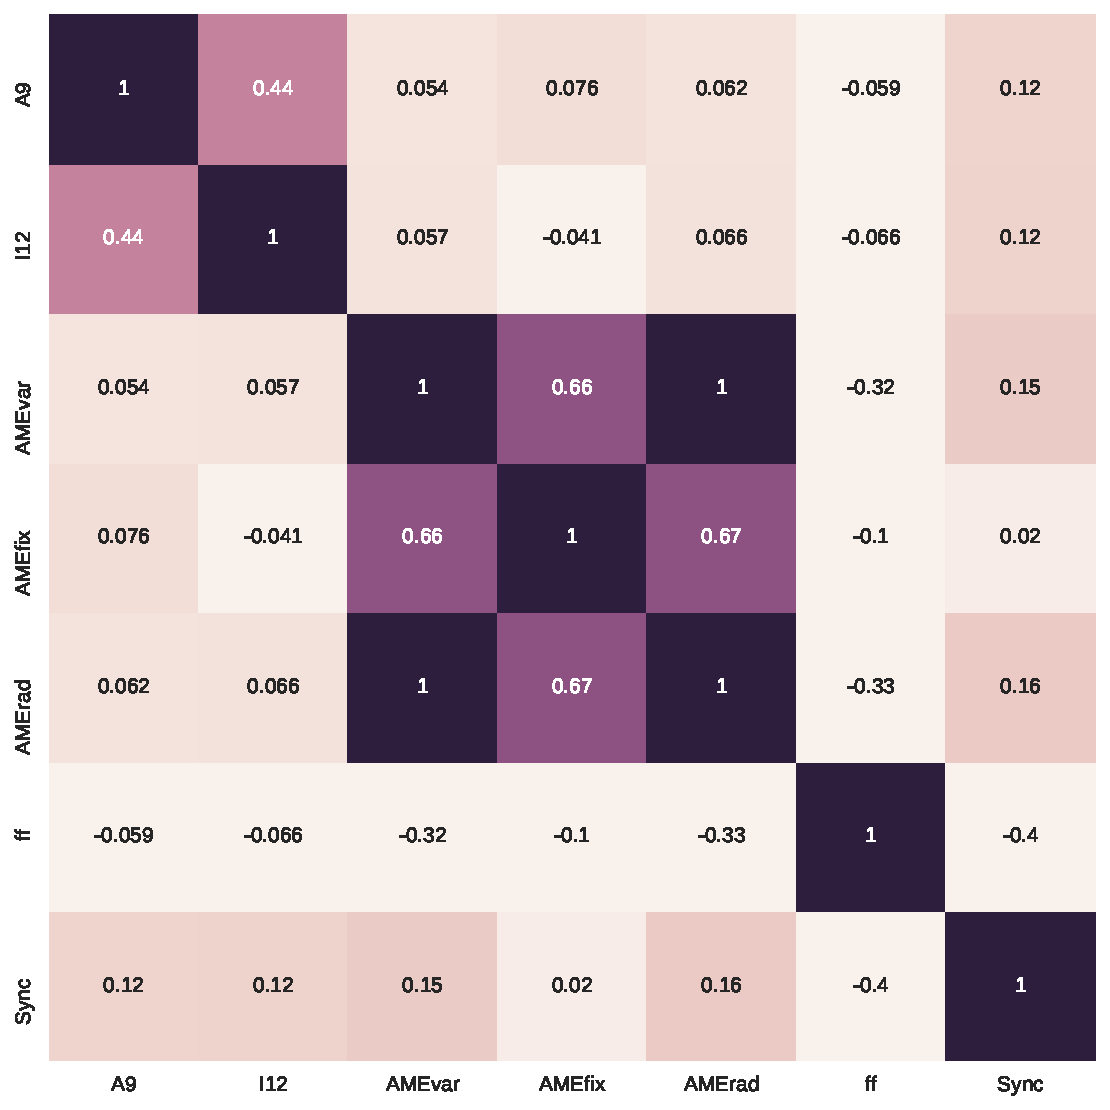
\includegraphics[width=\textwidth/2]{../Plots/ch_allsky/all_bands_corr_matrix_wAME_spearmanR_norm_masked_hens.pdf}
                    \centering
                    \caption{Cross-correlation ($r_{s}$ matrix for the residual correlations between IR intensities, \gls{ame}, and other microwave components. All of the maps in this case are normalized by $R$. )}
                    \label{fig:all_bands_corr_matrix_wAME_spearmanR_norm_masked_hens}
                \end{figure}
            As with the result in \cite{hensley16}, these data do not reveal any correlation between \gls{pah} fraction and $I_{AME}/R$, or with any of the MIR/R ratios and $I_{AME}/R$. Interestingly, there is evidence of a marginal positive trend with synchrotron, and a negative trend with free-free emission.

          \paragraph{Bootstrap test}
              In addition, for the masked comparison, we carry out a boostrap analysis, using the same method explained in Ch.~\ref{ch:intro} and implemented in Ch.~\ref{ch:lori}. The Spearman rank correlation coefficents $r_{S}$ of all of the bands, in intensity, vs. the $AME_{var}$ component are shown. This is done only for the masked case, due to the computational challeneges presented by a well-sampled bootstrap of all \textasciitilde{}780,000 pixels in the full sky. Because the mask applied here leaves us with approximately 7\% the sky, a bootstrap with $N_{iterations} > N_{pix}$ becomes tractable. We show the comparison only for the $AME_{var}$ component also due to computational constraints. The $r_{s}$ distributions for each IR band vs. \gls{ame} are shown in Fig.~\ref{fig:bootstrap_vs_AME_allsky_masked}.
                \begin{figure}
                     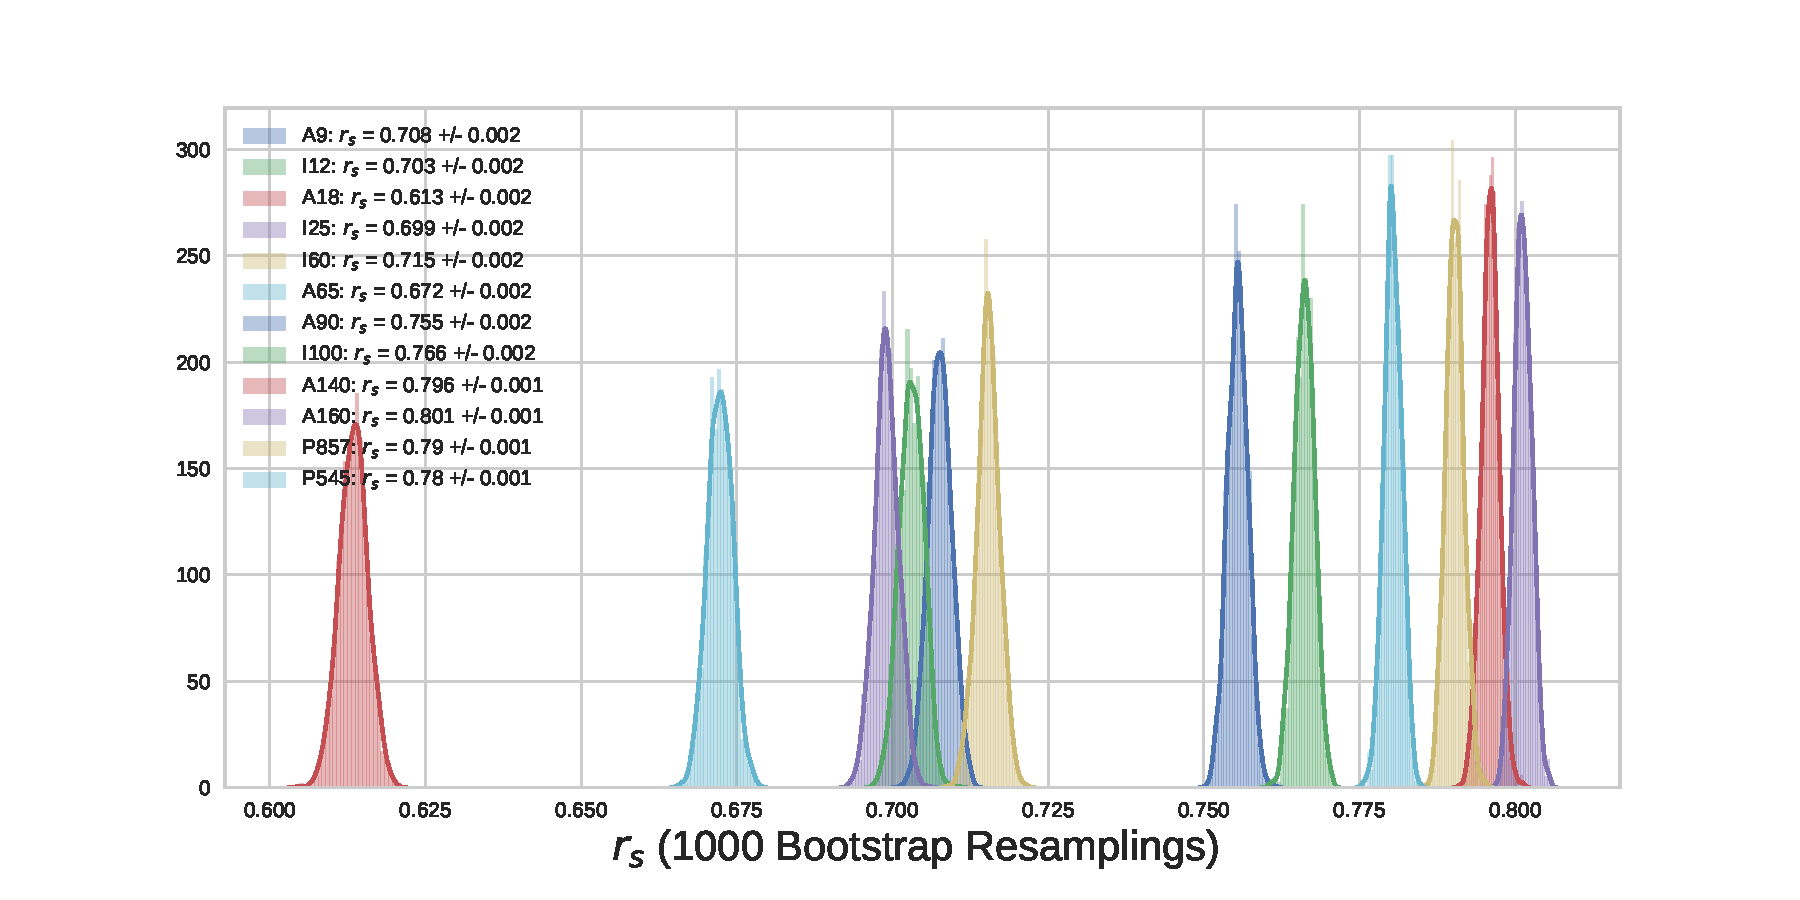
\includegraphics[width=\textwidth,trim={3cm 0.25cm 2.5cm 1cm},clip]{../Plots/ch_allsky/bootstrap_vs_AME_spearman_maskall_i1000.pdf}
                     \centering
                     \caption{Re-sampled (Bootstrap) correlation tests for IR emission vs. \gls{ame}, performed on the masked all-sky maps. Each band's $r_{s}$ distribution is shown in a different color. The width of the distribution indicates the error for the given data in the correlation coefficient. The mean and standard deviation of the scores are given in the legend of each plot. The plot ranges only show positive values, since no negative scores were produced. }
                     \label{fig:bootstrap_vs_AME_allsky_masked}
                \end{figure}
            The calculations are performed in the same way as with Fig.~\ref{fig:bootstrap_vs_AME} for $\lambda$~Orionis. Consistent with the other correlation analyses already shown in this chapter, there is a stronger correlation in the FIR, espeically A160. Considering the \gls{mir} range, and as with $\lambda$~Orionis, A9 emission correlates better than I12. The worst correlation is seen with the A18 and I25 bands.
\section{Spatial variation of correlations}
    To understand how these trends may vary across the sky, independent from the choice of pixel masl, we produce an all-sky maps of $r_{s}$ for \gls{ame} vs. IR emission. From the NSIDE~256 input maps of \gls{ame} and 4 IR wavelength maps, we produce NSIDE~8 maps of $r_{s}$. These maps are shown in Figs.~\ref{fig:Spearman_Map_nside8_AMEvartoIR_A9}-\ref{fig:Spearman_Map_nside8_AMEvartoIR_A140}
      \begin{figure}
        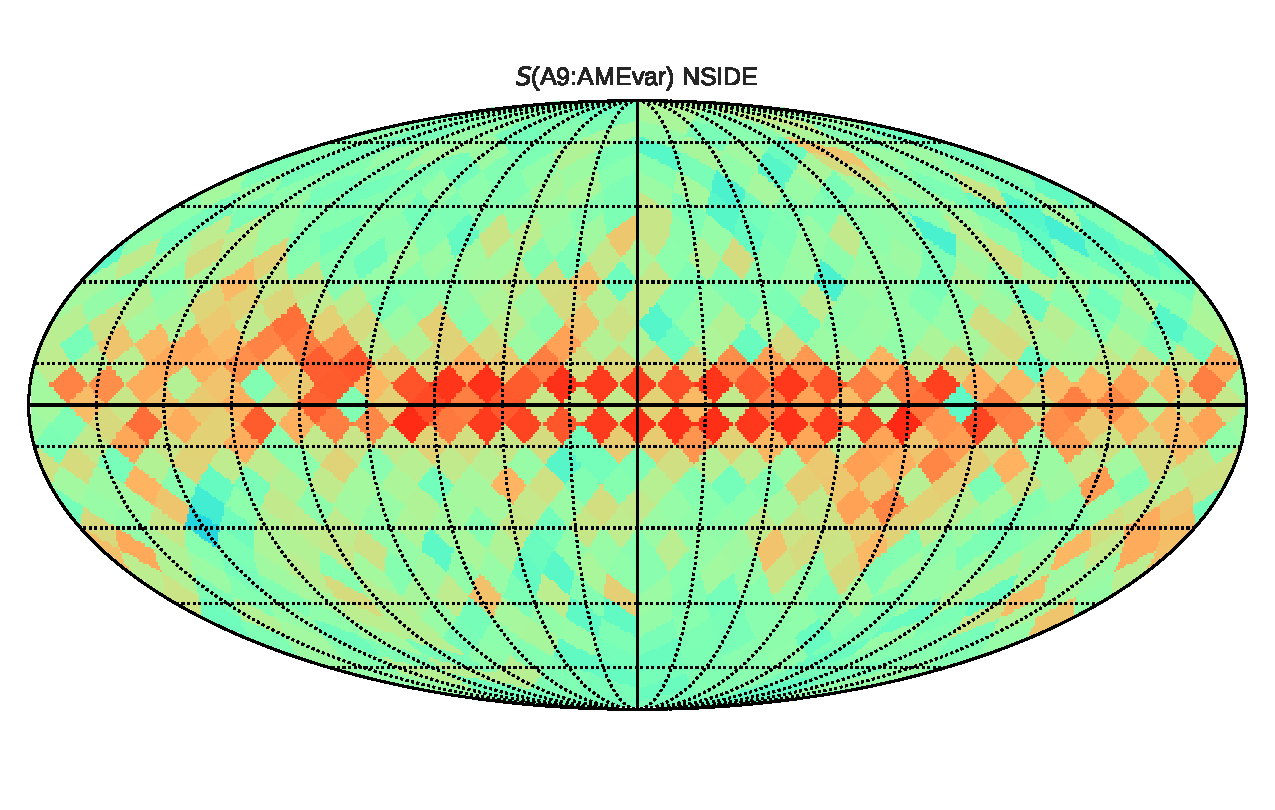
\includegraphics[width=\textwidth/2]{../Plots/Allsky_Corr/Spearman_Map_nside8_A9toAMEvar.pdf}
        \centering
        \caption{Spatial map of $r_{s}$ between the \gls{ame} and IR intensity for A9. $r_{s}$ is calculated for all NSIDE~256 pixels within each NSIDE~8 pixel-sized bin. The correlation score is calculated with the unmasked maps. The colorbar indicates $r_{s}$, ranging from -1 (negative monotonic relationship) to +1 (positive monotonic relationship).}
        \label{fig:Spearman_Map_nside8_AMEvartoIR_A9}
      \end{figure}
      \begin{figure}
        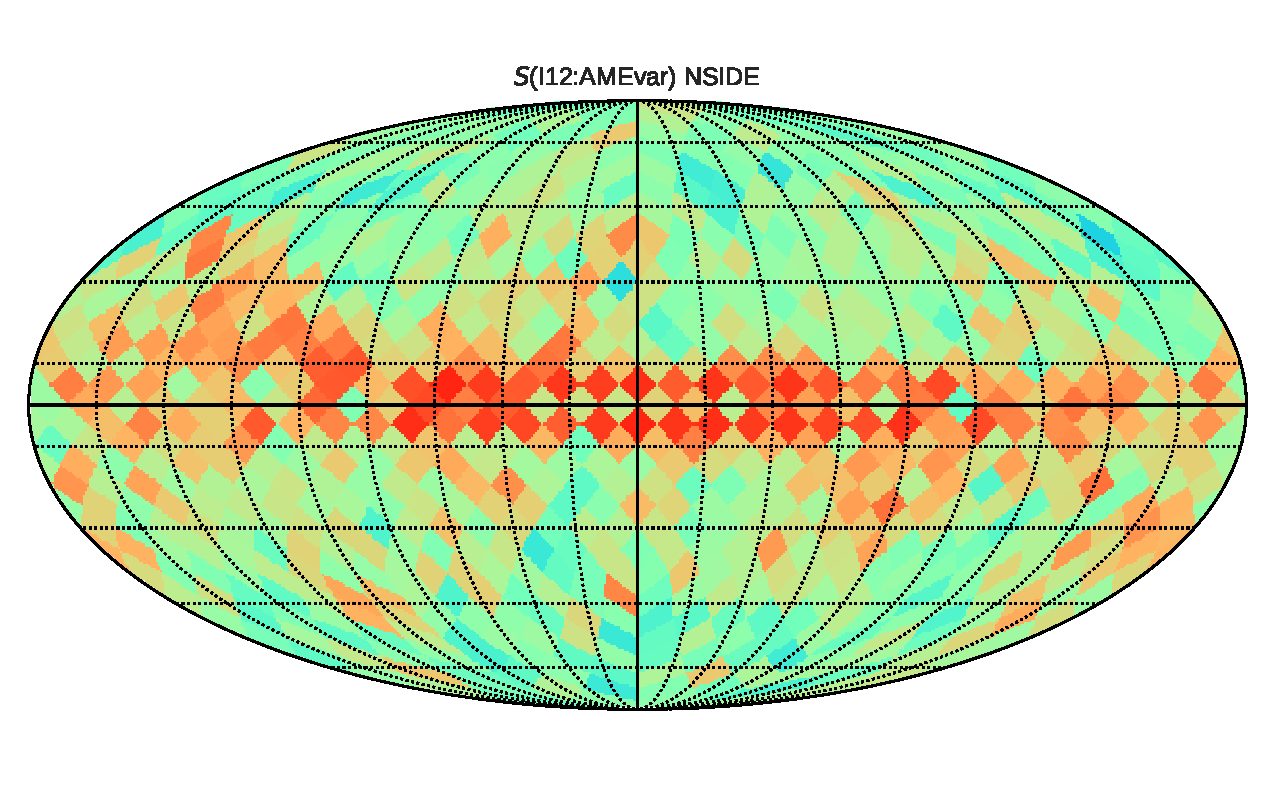
\includegraphics[width=\textwidth/2]{../Plots/Allsky_Corr/Spearman_Map_nside8_I12toAMEvar.pdf}
        \centering
        \caption{Spatial map of $r_{s}$ between the \gls{ame} and IR intensity for I12, calculated as in Fig.~\ref{fig:Spearman_Map_nside8_AMEvartoIR_A9}.}
        \label{fig:Spearman_Map_nside8_AMEvartoIR_I12}
      \end{figure}
      \begin{figure}
        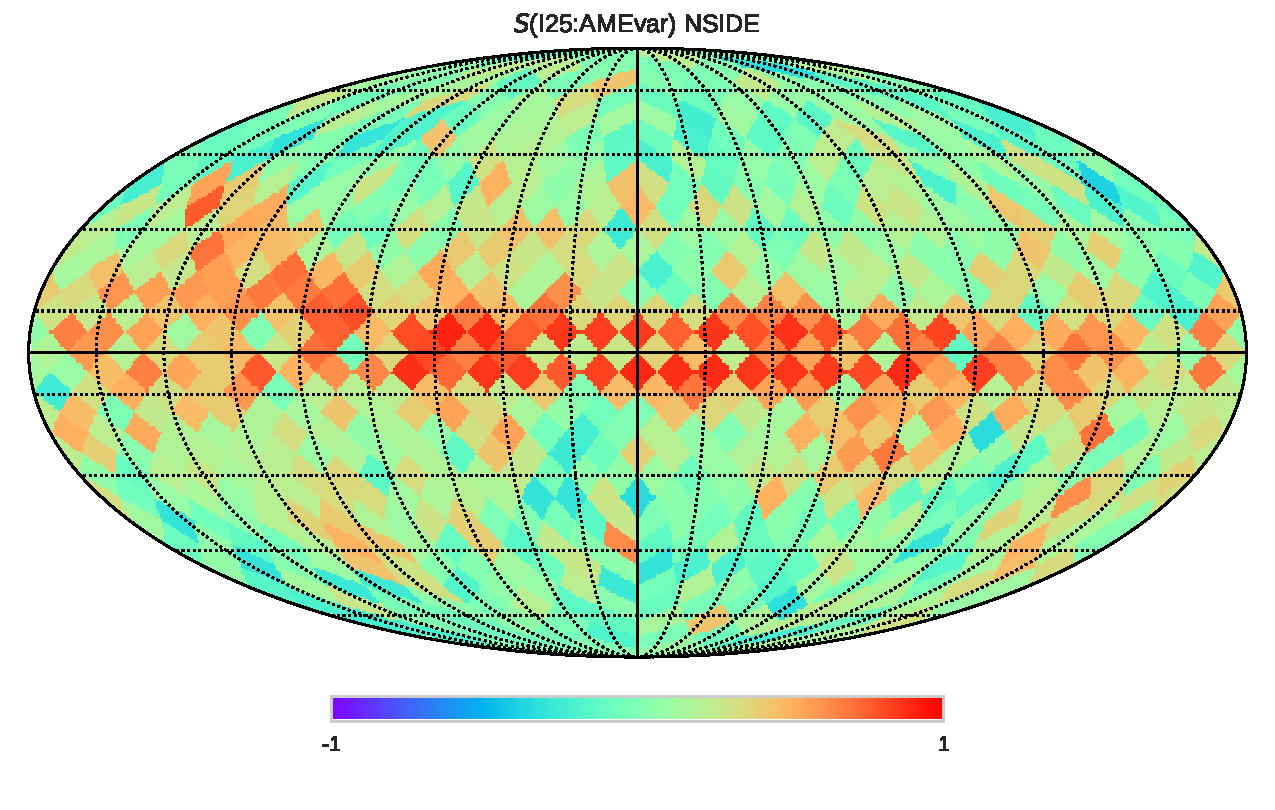
\includegraphics[width=\textwidth/2]{../Plots/Allsky_Corr/Spearman_Map_nside8_I25toAMEvar.pdf}
        \centering
        \caption{Spatial map of $r_{s}$ between the \gls{ame} and IR intensity for I25, calculated as in Fig.~\ref{fig:Spearman_Map_nside8_AMEvartoIR_A9}.}
        \label{fig:Spearman_Map_nside8_AMEvartoIR_I25}
      \end{figure}
      \begin{figure}
        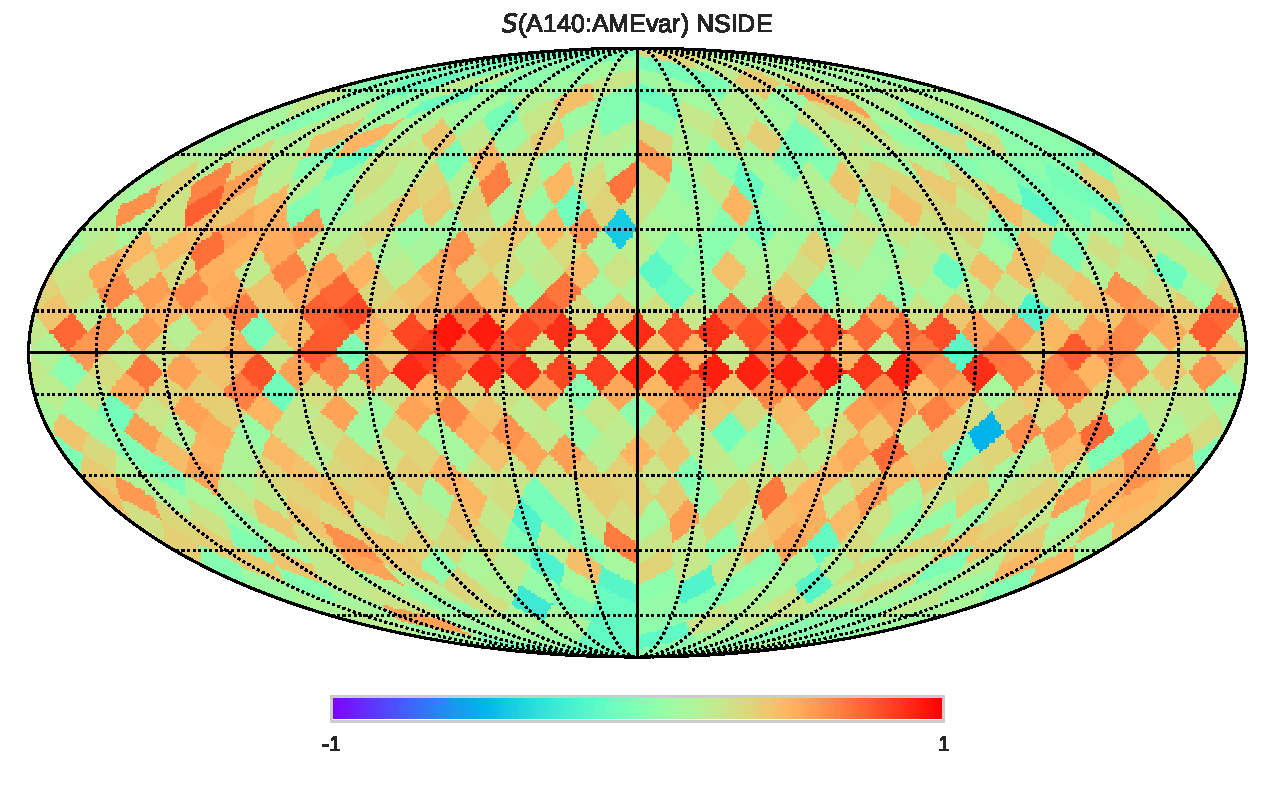
\includegraphics[width=\textwidth/2]{../Plots/Allsky_Corr/Spearman_Map_nside8_A140toAMEvar.pdf}
        \centering
        \caption{Spatial map of $r_{s}$ between the \gls{ame} and IR intensity for A140, calculated as in Fig.~\ref{fig:Spearman_Map_nside8_AMEvartoIR_A9}.}
        \label{fig:Spearman_Map_nside8_AMEvartoIR_A140}
      \end{figure}
  The most important feature of these maps is that they look very similar, confirming in a spatial context that there is very little difference overall, when comparing \gls{ame} to IR in intensity, accross multiple wavelengths. The correlations weaken for the \gls{mir} bands at higher latitudes, as expected. Thus the question of which band correlates better depends on exactly where we look. Considering that we need also to look at secondary correlations, not only in intensity, we repeat the above process for ratios of the \gls{mir} to \gls{ame}, scaling both by $U$, as in Fig,~\ref{fig:all_bands_corr_matrix_wAME_spearmanU_norm_masked}.  Figs.~\ref{fig:Spearman_Map_nside8_AMEvartoIR_UNorm_A9}-\ref{fig:Spearman_Map_nside8_AMEvartoIR_UNorm_I25} show such correlation maps.
     \begin{figure}
       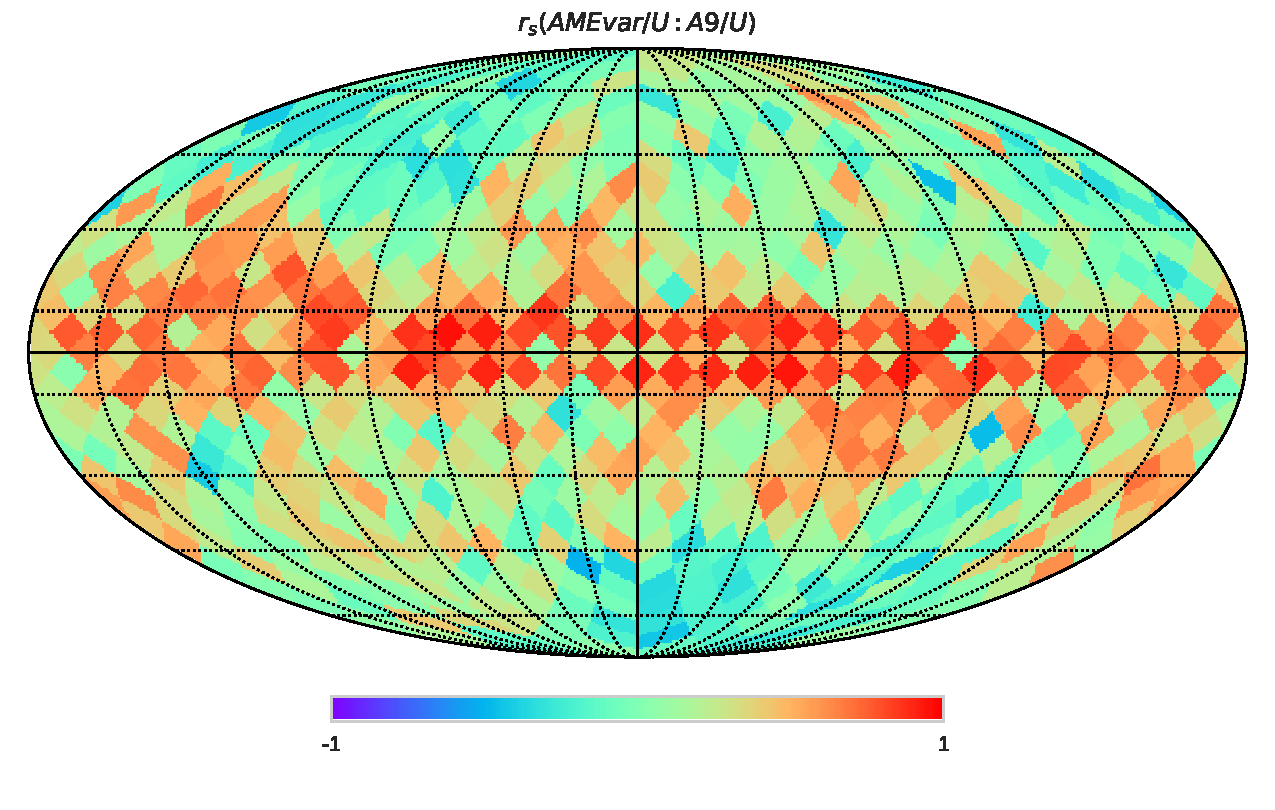
\includegraphics[width=\textwidth/2]{../Plots/Allsky_Corr/UNorm/Spearman_Map_nside8_AMEvartoA9.pdf}
       \centering
       \caption{Spatial map of $r_{s}$ between the \gls{ame}:$U$ and A9:$U$, a tracer of the column density of \gls{pah}s emitting within the A9 filter. The correlations are calculated as in Fig.~\ref{fig:Spearman_Map_nside8_AMEvartoIR_A9}.}
       \label{fig:Spearman_Map_nside8_AMEvartoIR_UNorm_A9}
     \end{figure}
     \begin{figure}
       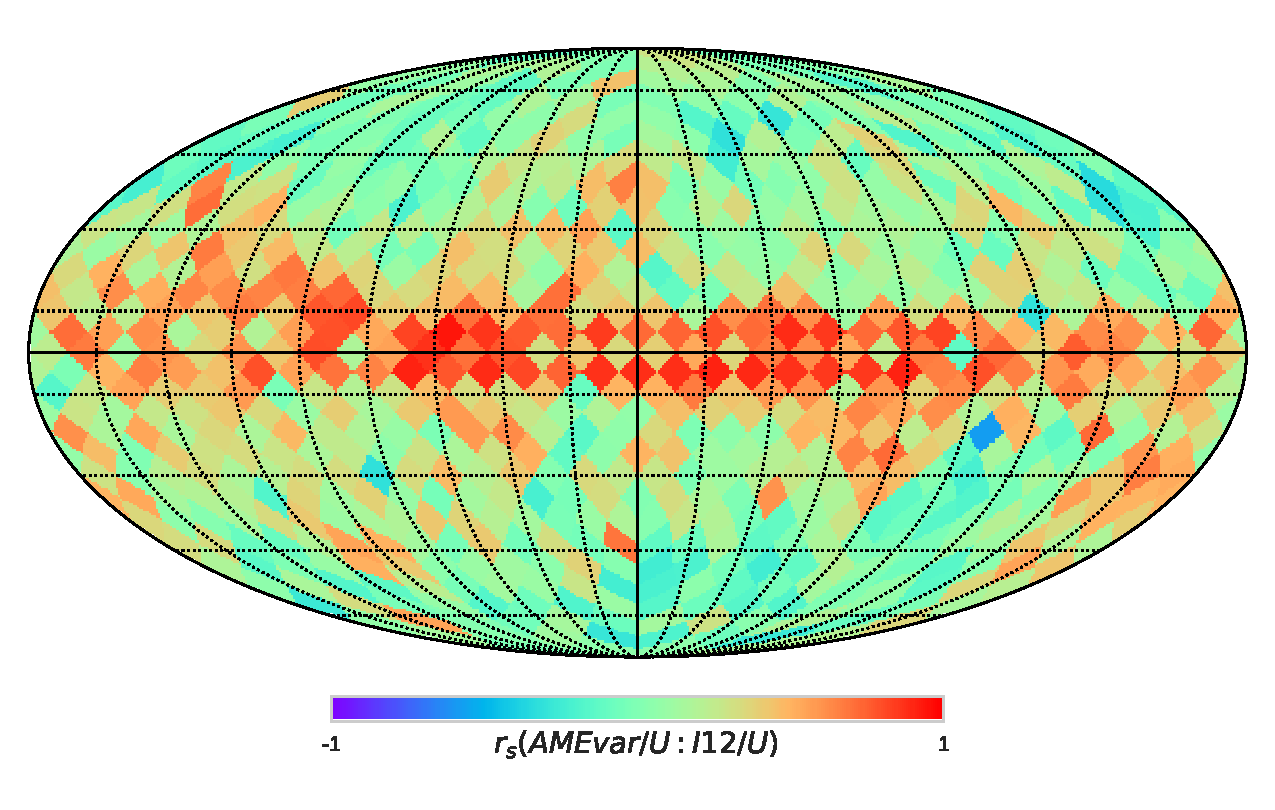
\includegraphics[width=\textwidth/2]{../Plots/Allsky_Corr/UNorm/Spearman_Map_nside8_AMEvartoI12.pdf}
       \centering
       \caption{Spatial map of $r_{s}$ between the \gls{ame}:$U$ and I12:$U$}
       \label{fig:Spearman_Map_nside8_AMEvartoIR_UNorm_I12}
     \end{figure}
      \begin{figure}
        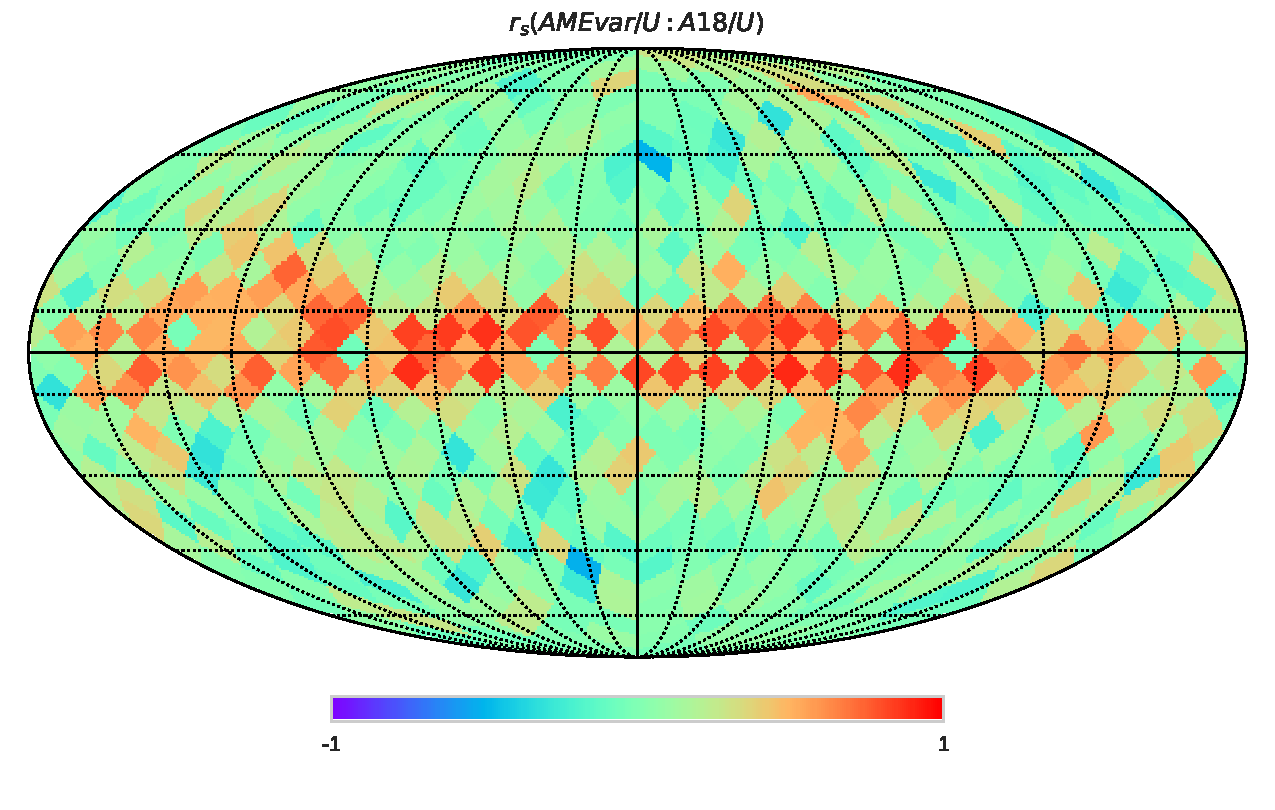
\includegraphics[width=\textwidth/2]{../Plots/Allsky_Corr/UNorm/Spearman_Map_nside8_AMEvartoA18.pdf}
        \centering
        \caption{Spatial map of $r_{s}$ between the \gls{ame}:$U$ and A18:$U$}
        \label{fig:Spearman_Map_nside8_AMEvartoIR_UNorm_A18}
      \end{figure}
    \begin{figure}
         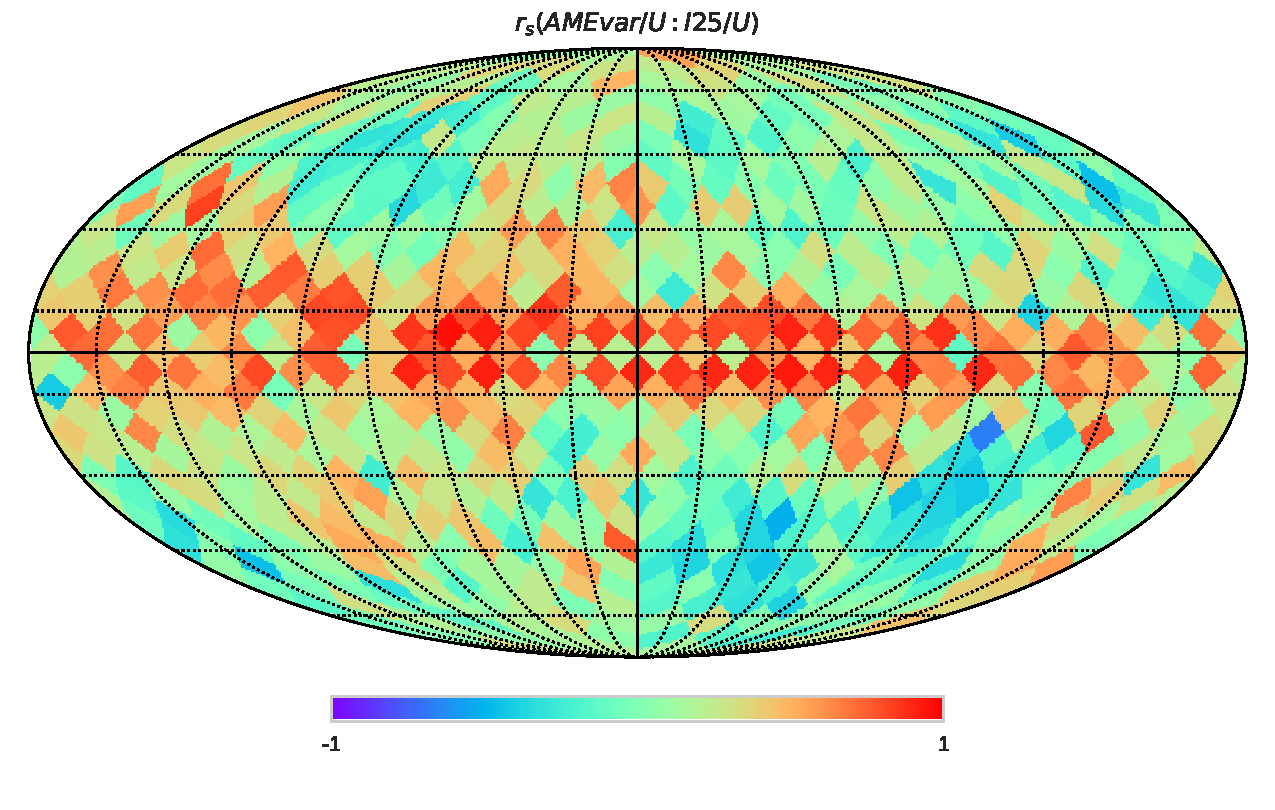
\includegraphics[width=\textwidth/2]{../Plots/Allsky_Corr/UNorm/Spearman_Map_nside8_AMEvartoI25.pdf}
         \centering
         \caption{Spatial map of $r_{s}$ between the \gls{ame}:$U$ and I25:$U$}
         \label{fig:Spearman_Map_nside8_AMEvartoIR_UNorm_I25}
    \end{figure}
  Scaling by $U$ does not change the overall structure of these correlation maps, relative to the unscaled versions. This may indicate that at the scale of these correlation maps, the strength of $U$ does not show much variation.

    \section{Discussion}
        As noted in Ch.~\ref{ch:intro}, previous studies found that the \gls{ame} generally correlates at dust-related IR wavelengths \citep{ysard10b,planckXV, hensley16}. We see the same overall pattern in the present study. We also corroborate that the FIR emission shows the tightest correlation with the \gls{ame} intensity, for large portion of the sky in a de-localized fashion (Figs.~\ref{fig:all_bands_corr_matrix_wAME_spearman} and~ \ref{fig:all_bands_corr_matrix_wAME_spearmanintensity_maskall}). In testing for a second-order correlation, we divided the IR intensities and \gls{ame} intensity by $U$, and again performed the band-by-band all-sky comparison. There is evidence of a residual correlation between $I_{MIR}/U$ and $I_{AME}/U$ (Figs.~\ref{fig:all_bands_corr_matrix_wAME_spearmanU_norm_masked}, and~\ref{fig:Spearman_Map_nside8_AMEvartoIR_UNorm_A9}-\ref{fig:Spearman_Map_nside8_AMEvartoIR_UNorm_I25}).

       The closeness of the correlation coefficients found here is consistent with the results of the IRAS vs. \gls{ame} correlation test result from \cite{planckXV}. They found that the correlation coefficient among the four IRAS bands (12, 25, 60, and 100~$\mu$m) differ from one another only by about 5\%, across their whole set of 98 regions. They had also indicated that many of the regions sampled were HII regions, and that free-free emission may not have been completely separated from the \gls{ame}. We consider that a similar phenomenon may be happening in the PCAME map we explore here. The trend of AKARI \gls{mir} and FIR data vs. the \gls{ame} does not disagree with their IRAS comparison. This work adds that individual band intensities longer than IRAS 100~$\mu$m also correlate strongly with \gls{ame}, especially the two Planck/HFI bands used.

          \subsection{AME and interstellar radiation fields}
            In our masked analysis, we were unable to replicate with the PC data a result by \cite{ysard10b} wherein scaling the \gls{mir} bands by $U$ improves the correlation of \gls{mir} vs. \gls{ame}. Instead we found that the best correlation between the \gls{mir} bands and \gls{ame} is found after scaling both by $U$. There is a chance that this improvement is induced by the common division of noise-terms in $U$, but if this correlation increase is real it may indicate that the \gls{ame} intensity is somewhat dependent on $U$. While it is expected that \gls{ame} intensity depends both on the abundance of carriers, and various excitation terms, it is not predicted that $U$ directly influences spinning dust excitation. However it may be an indirect tracer of galactic environments and various other spinning dust excitation factors. he slight improvement with division by $U$ was also seen with our investigation of $\lambda$~Orionis in Ch.~\ref{ch:lori}.

            According to spinning dust theory outlined in \cite{draine98a} and in subsequent works by \cite{ysard10a}, the \gls{ame} profile and intensity will depend in part on the ISRF- but as is well-stated in \cite{hensley17a}, exactly how the ISRF will affect the \gls{ame} \gls{sed} is a more complicated question. Absorbed starlight photons may be able to rotationally excite the carriers, but if an enhanced ISRF leads to increased dust heating, then the increased IR emission can rotationally de-excite the carriers. Moreover the ISRF affects not only the dust temperature but ionization of the carriers.

          \subsection{Microwave foreground component separation}
            There are known degeneracies between the foreground parameters of the COMMANDER maps (spinning-dust, and free-free, synchrotron components as described in \cite{planck15X}.) This can be demonstrated by examining the ratio map of the \gls{ame} intensity to $R$, in comparison with the \gls{pc} free-free and synchrotron maps. Figs.~\ref{fig:AMEvartoDust_ffandSyncCountours} and~\ref{fig:AMEfixtoDust_ffandSyncCountours} show the $AME_{var}/R$ and $AME_{fix}/R$ ratio maps, with contours from the free-free and synchrotron maps.
                \begin{figure}
                    
\includegraphics[width=\textwidth,trim={6cm 2cm 5.0cm 2cm},clip]{../Plots/ch_allsky/AMEvartoDust_ffandSyncCountours.pdf}
                    \centering
                    \caption{The ratio of $AME_{var}$ and PC dust radiance $R$, tracing fluctuations in \gls{ame} per thermal dust emission. The contours trace the PC synchrotron (black) and free-free (white) components, to highlight various correlations between these components and PC \gls{ame} fluctuations. Both free-free and syhncrotron can be seen to correlate and anti-correlate with the \gls{ame} to dust ratio.}
                    \label{fig:AMEvartoDust_ffandSyncCountours}
                \end{figure}
                \begin{figure}
                    
\includegraphics[width=\textwidth,trim={6cm 2cm 5.0cm 2cm},clip]{../Plots/ch_allsky/AMEfixtoDust_ffandSyncCountours.pdf}
                    \centering
                    \caption{The same as Fig.~\ref{fig:AMEvartoDust_ffandSyncCountours}, but with $AME_{fix}/R$ as the all-sky image.}
                    \label{fig:AMEfixtoDust_ffandSyncCountours}
                \end{figure}
             There are clearly regions where synchrotron emission correlates with \gls{ame} excesses. Some of these appear as more large scale fluctuations, mainly at higher galactic latitude. Interestingly, free-free shows agreement with both positive and negative fluctuations in both ratio maps. At high galactic latitude, free-free tends to be associated with positive fluctuations. This is supported by the fact that $AME_{fix}$ shows an improved correlation with both the $H\alpha{}$ map and the PC free-free map, perhaps suggesting confusion between spinning dust and free-free components. Interestingly, the ring-structure of the $\lambda$~Orionis region analyzed in Ch.~\ref{ch:lori}, does not have any apparent conterpart in the $AME/R$ ratio maps in Figs.~\ref{fig:AMEfixtoDust_ffandSyncCountours}~and~\ref{fig:AMEvartoDust_ffandSyncCountours}.

             The results of the $R$ normalized cross-correlation test show that free-free/R shows a negative correlation with $AME/R$. This may be furher indication that the \gls{ame} map, even with the mask applied from Sec.\ref{sec:pixmask}, may suffer from significant MW component confusion in some regions. It is difficult to quantify potential effects from component separation uncertainties relative to genuine correlations between microwave emission components, with the present data. However there remains the potential for such confusion to suppress evidence of any trend between \gls{ame} and the actual value of $fPAH$. The anti-correlation here between free-free/R and \gls{ame}/R may be consistent with findings in \cite{vonHausegger15} that free-free emission anti-correlates with \gls{ame}, if pixels are weighted by \gls{sn}.

             Even though A9/R and I12/R do not correlate with \gls{ame}/R in our masked comparison, we do find some limited regions where these values correlate in our full spatial correlation mapping.

            \subsection{Optical depth}
              In the interpretation of results here, we have essentially operated under the assumption that MIR/PAH emisison, FIR emission, and the \gls{ame} are all in the optically thin domain. This is supported by the strong agreement in $r_{s}$, accross all IR bands and the \gls{ame}, as presented in the correlation matrices here. (With the exception of the high-latitude, unmasked case in Fig~\ref{fig:all_bands_corr_matrix_wAME_spearman}.) Conversely, the $H{\alpha}$ data --- emission known to be absorbed by interstellar dust --- is the only map lacking a correlation with the others at $|\beta{}|<5^{\circ}$. $N(H)$ also shows a weaker correlation nearer to the galactic plane, likely influenced by saturation and/or self-absorption effects.

              However it has been demonstrated by \cite{sakon04} that the optically-thin assumption for \gls{pah}/UIR emission could lead to errors in the estimate of \gls{pah} abundance based on these emision features. Self-absorption for \gls{pah}s is another possibility.

              We do not expect the analysis presented here to suffer from such effects significantly, as we have masked the most confused lines of sight towards the galactic plane. However we cannot rule out the possibility that such optical depth effects, not only in \gls{pah} emisison but in the FIR or even \gls{ame}, may weaken any potential relationship between the IR and microwave emisison from spinning grains.

            \subsection{Comparison of $\lambda$~Orionis vs. All-sky results}
              Results presented here do not necessarily conflict with results from Ch.~\ref{ch:lori}, except in that the findings from Fig.~\ref{fig:bootstrap_vs_AME}, wherein $r_{p}$ of A9 emission correlates better with \gls{ame} than P545 emission, do not generalize to the results of this chapter (either the masked or unmasked cases.) However, in the masked all-sky comparison as well as in $\lambda$~Orionis, we find a better corrleation between A9 and \gls{ame} than between I12 and \gls{ame} when we subject the correlations to bootstrap resampling.

               The different results between Ch.~\ref{ch:lori} and Ch.~\ref{ch:allsky} may be explained by variations in the component separation reliability. It is apparent that with the presently available data, there are a very limited number of regions on the sky which do not show strong free-free or synchrotron emission (relative to \gls{ame}), while also having enough \gls{sn} in the \gls{mir} to reliably probe a relationship between \gls{pah} abundance fluctuations and \gls{ame} fluctuations. $\lambda$~Orionis may be one of the exceptions, where the \gls{sn} is high enough, and we are in fact able to see an improved correlation between \gls{pah}s and \gls{ame}, relative to the overall dust emission to \gls{ame} connection.

              We also disucssed in Ch.~\ref{ch:allsky} the possibility that the \gls{pah} emission may not necessarily be optically thin. If this were true, it may explain discrepancies for our $\lambda$~Orionis result and the results in this chapter. $\lambda$~Orionis provides us a relatively clean line of sight compared to delocalized all-sky analysis.

              The fact that we do not see a clear preferential relationship between \gls{ame} and \gls{pah}s in the all-sky analysis, does not rule out a contribution by spinning \gls{pah}s to the \gls{ame}. Likewise the fact that we do see a better correlation in $\lambda$~Orionis does not rule out contributions from other proposals, such as that form non-PAH small grains, or nanosilicates.


              \subsection{Implications of an absent \gls{pah}-AME correlation}
                  In the case that we are able to rule \gls{pah}s out as the \gls{ame} carrier with confidence, this may imply some constraints on the \gls{pah} size distribution and dipole moment. As discussed in the theoretical work by \cite{draine98a, ali-haimoud10} and others, as well as the observational work by \cite{hensley16}, if \gls{pah}s exist in the \gls{ism}, they are very likely to be spinning rapidly. Thus if we are able to confirm that they do not produce \gls{ame}, this could tell us the morphology of \gls{ism} \gls{pah}s are not in an appropriate range to produce the observed \gls{ame}. Spinning \gls{pah}s may be a reality even in the case that the \gls{ame} comes from something else, if the \gls{pah}s are too large or lack appropriate electric dipoles.

              \section{Future Works}
                  Because of the issues highlighted in previous sections (S/N, component separation, etc.), it is extremely difficult to draw a conclusion about the carrier of \gls{ame} based on a general all-sky analysis such as that shown here. However there may be promise in studies of individual regions, where an attempt can be made at controlling for local environmental factors, or background/foreground contamination. While it is true that previous studies of specific objects have also not been conclusive, such as the investigation of Perseus by \cite{tibbs11}, there are still many other \gls{ame} prominent regions which have not been probed in-depth, through a combination of microwave and \gls{pah}-range observations. Even the study of $\lambda$~Orionis in Ch.~\ref{ch:lori} is not exhaustive, and this interesting region deserves further attention from targeted observations.

                New tests of \gls{ame} hypotheses should: push limitations in the available data and, focus on regions well-documented to show a spinning-dust-like \gls{ame} spectrum. While a simple excess of microwave emission may be able to be fit by a spinning dust model \gls{sed}, the spinning dust explanation is not testable unless the observed \gls{sed} shows evidence of a low-frequency downturn.

                There are two major boundaries that, based on results presented here, must be pushed. Spatial resolution and spectral coverage.
                Spatial resolution constraints are a critical issue in multiwavelength astornomy, especially in dust-related works. To explain why, simply consider the description of dust research from Ch.~\ref{ch:intro}, and Tab.~\ref{tab:data}. The spatial resolution of available data has a wide discrepancy from the \gls{mir} to microwave: ~10 arcseconds for AKARI 9 micron to at least a degree FWHM for the ``effective resolution'' of parameter maps. Likewise, if there are enivonmental diffrences only visible at sub-degree angular scales, we will have a hard time controlling for the excitation factors of spinning dust emission. Without separating excitation factors from column density of the carriers. Pairing opportunities for resolution maximizing ground-based observations of very limited regions of the sky, utilizing facilities such as the Atacama Large Milimeter Array (ALMA) Band 1 (30-35~GHz, still in production, \cite{huang16}.), with detailed assesment of tracers of small dust grains, will be helpful.

                Future breakthroughs in the \gls{ame} may be seen if we are able to increase the number of regions with a reliable \gls{ame} estimation. This can be obtained through improved synchrotron emission constraints, at higher resolutions. \gls{cbass} at 5~GHz will be helpful in this regard \citep{irfan15}. \gls{cbass} is expected to provide higher resolution low frequency constraints for the whole sky (48$'$ compared to 56$'$ for $H408$), with improved sensitivity (0.1~$\mu$K). In terms of localized studies, it may be fruitful to consider the physical environment of each region (i.e. ionization state, gas temperature and density, other conditions indicated in \cite{draine98a, ali-haimoud10} to affect the \gls{sed} shape) rather than relying of frequency-shifts to a template spectrum. More detailed exploration of \gls{pah} ionization, and other fluctuations between individual \gls{pah} features relative to variations in the \gls{ame} spectral profile may also help us understand potential roles of \gls{pah}s in producing \gls{ame}. However, even if we have excellent constraints on \gls{pah} emission features, synchrotron emission, free-free emission, and a powerful spinning dust \gls{sed} model, the key data will be spectral coverage of the full \gls{ame} profile. As noted in Ch.~\ref{ch:datasources}, the all-sky maps currently available, do not give constraints in the 10-20~GHz range. This means that lower frequency spinning dust peaks and emissivities are not well known. Improved understanding of \gls{ame} and spinning dust therefore will require observations such as those being undertaken by the Q-U-I JOint Tenerife Experiment (QUIJOTE) project, which offers coverage between 10 and 20~GHz \citep{santos15}.
